\documentclass[tikz, 12pt]{report}
\usepackage[utf8]{inputenc}
\usepackage[margin=20mm]{geometry}
\usepackage[pdfborder={0 0 0},backref=page]{hyperref}
\usepackage{dissertation}
\usepackage{lineno}
\linespread{1.5}

\hypersetup{
    colorlinks=true,
    urlcolor=blue,
    linkcolor=black,
    citecolor=blue!70!black,
}

\bibliographystyle{apalike}

\title{{ 
\includegraphics[scale=.5]{figures/ucl_logo.png}}\\
{{\Huge Does Size Matter?}\\{\Large The Effect of Sample Size on Steering}}\\
}
\date{Submission date: 8 September 2025}
\author{PRHC8\thanks{
{\bf Disclaimer:}
This report is submitted as part requirement for the Machine Learning MSc at UCL. It is
substantially the result of my own work except where explicitly indicated in the text.
The report may be freely copied and distributed provided the source is explicitly acknowledged}
\\ \\
Machine Learning MSc\\ \\
Daniel Tan \& Brooks Paige}

\begin{document}
\linenumbers

%TC:ignore
%%%%% NEW MATH DEFINITIONS %%%%%

% Mark sections of captions for referring to divisions of figures
\newcommand{\figleft}{\em (Left)}
\newcommand{\figcenter}{\em (Center)}
\newcommand{\figright}{\em (Right)}
\newcommand{\figtop}{\em (Top)}
\newcommand{\figbottom}{\em (Bottom)}
\newcommand{\captiona}{\em (a)}
\newcommand{\captionb}{\em (b)}
\newcommand{\captionc}{\em (c)}
\newcommand{\captiond}{\em (d)}

% Highlight a newly defined term
\newcommand{\newterm}[1]{\mathbf #1}

\def\ceil#1{\lceil #1 \rceil}
\def\floor#1{\lfloor #1 \rfloor}
\def\1\mathbf{1}
\newcommand{\train}{\mathcal{D}}
\newcommand{\valid}{\mathcal{D\_\mathrm{valid}}}
\newcommand{\test}{\mathcal{D\_\mathrm{test}}}

\def\eps{\epsilon}

% Vectors
\def\vzero{\mathbf{0}}
\def\vone{\mathbf{1}}
\def\vmu{\mathbf{\mu}}
\def\vtheta{\mathbf{\theta}}
\def\va{\mathbf{a}}
\def\vb{\mathbf{b}}
\def\vc{\mathbf{c}}
\def\vd{\mathbf{d}}
\def\ve{\mathbf{e}}
\def\vf{\mathbf{f}}
\def\vg{\mathbf{g}}
\def\vh{\mathbf{h}}
\def\vi{\mathbf{i}}
\def\vj{\mathbf{j}}
\def\vk{\mathbf{k}}
\def\vl{\mathbf{l}}
\def\vm{\mathbf{m}}
\def\vn{\mathbf{n}}
\def\vo{\mathbf{o}}
\def\vp{\mathbf{p}}
\def\vq{\mathbf{q}}
\def\vr{\mathbf{r}}
\def\vs{\mathbf{s}}
\def\vt{\mathbf{t}}
\def\vu{\mathbf{u}}
\def\vv{\mathbf{v}}
\def\vw{\mathbf{w}}
\def\vx{\mathbf{x}}
\def\vy{\mathbf{y}}
\def\vz{\mathbf{z}}

% Matrix
\def\mA{\mathbf{A}}
\def\mB{\mathbf{B}}
\def\mC{\mathbf{C}}
\def\mD{\mathbf{D}}
\def\mE{\mathbf{E}}
\def\mF{\mathbf{F}}
\def\mG{\mathbf{G}}
\def\mH{\mathbf{H}}
\def\mI{\mathbf{I}}
\def\mJ{\mathbf{J}}
\def\mK{\mathbf{K}}
\def\mL{\mathbf{L}}
\def\mM{\mathbf{M}}
\def\mN{\mathbf{N}}
\def\mO{\mathbf{O}}
\def\mP{\mathbf{P}}
\def\mQ{\mathbf{Q}}
\def\mR{\mathbf{R}}
\def\mS{\mathbf{S}}
\def\mT{\mathbf{T}}
\def\mU{\mathbf{U}}
\def\mV{\mathbf{V}}
\def\mW{\mathbf{W}}
\def\mX{\mathbf{X}}
\def\mY{\mathbf{Y}}
\def\mZ{\mathbf{Z}}
\def\mBeta{\mathbf{\beta}}
\def\mPhi{\mathbf{\Phi}}
\def\mLambda{\mathbf{\Lambda}}
\def\mSigma{\mathbf{\Sigma}}

% Sets
\def\sA{\mathcal{A}}
\def\sB{\mathcal{B}}
\def\sC{\mathcal{C}}
\def\sD{\mathcal{D}}
\def\sE{\mathcal{E}}
\def\sF{\mathcal{F}}
\def\sG{\mathcal{G}}
\def\sH{\mathcal{H}}
\def\sI{\mathcal{I}}
\def\sJ{\mathcal{J}}
\def\sK{\mathcal{K}}
\def\sL{\mathcal{L}}
\def\sM{\mathcal{M}}
\def\sN{\mathcal{N}}
\def\sO{\mathcal{O}}
\def\sP{\mathcal{P}}
\def\sQ{\mathcal{Q}}
\def\sR{\mathcal{R}}
\def\sS{\mathcal{S}}
\def\sT{\mathcal{T}}
\def\sU{\mathcal{U}}
\def\sV{\mathcal{V}}
\def\sW{\mathcal{W}}
\def\sX{\mathcal{X}}
\def\sY{\mathcal{Y}}
\def\sZ{\mathcal{Z}}

\newcommand{\E}{\mathbb{E}}
\newcommand{\Ls}{\mathcal{L}}
\newcommand{\R}{\mathbb{R}}
\newcommand{\N}{\mathbb{N}}
\newcommand{\emp}{\tilde{p}}
\newcommand{\lr}{\alpha}
\newcommand{\reg}{\lambda}
\newcommand{\rect}{\mathrm{rectifier}}
\newcommand{\softmax}{\mathrm{softmax}}
\newcommand{\sigmoid}{\sigma}
\newcommand{\softplus}{\zeta}
\newcommand{\KL}{D\_\mathrm{KL}}
\newcommand{\Var}{\mathrm{Var}}
\newcommand{\standarderror}{\mathrm{SE}}
\newcommand{\Cov}{\mathrm{Cov}}
% Wolfram Mathworld says $L^2$ is for function spaces and $\ell^2$ is for vectors
% But then they seem to use $L^2$ for vectors throughout the site, and so does
% wikipedia.
\newcommand{\normlzero}{L\^0}
\newcommand{\normlone}{L\^1}
\newcommand{\normltwo}{L\^2}
\newcommand{\normlp}{L\^p}
\newcommand{\normmax}{L\^\infty}

\newtheorem{theorem}{THEOREM}
\newtheorem{lemma}[theorem]{LEMMA}
\newtheorem{corollary}[theorem]{COROLLARY}
\newtheorem{proposition}[theorem]{PROPOSITION}
\newtheorem{remark}[theorem]{REMARK}
\newtheorem{definition}[theorem]{DEFINITION}
\newtheorem{fact}[theorem]{FACT}

\newtheorem{problem}[theorem]{PROBLEM}
\newtheorem{exercise}[theorem]{EXERCISE}
\def \set#1{\{#1\} }

\newenvironment{proof}{
PROOF:
\begin{quotation}}{
$\Box$ \end{quotation}}

\newcommand{\mfullname}{Skye Purchase}
\newcommand{\mtitle}{As Yet Untitled}
\newcommand{\mdate}{\today}
\newcommand{\msupervisor}{}


\pagenumbering{roman}

\onehalfspacing
\maketitle

\chapter*{Acknowledgements}

I want to thank my family, especially my mum and dad who have supported me throughout my life and encouraged me to explore the world.
To my wider family who have both directly and indirectly supported me throughout the masters.

Particular thanks goes to Mia who has supported me throughout the highs and lows, stress and anxiety of the masters and the year leading up to it.
Thank you for listening to my endless rambles about the project and all the other projects I've had; keeping me focused, motivated, and on track to complete the thesis.

I would like to thank my supervisor Daniel Tan and the support of the ML Alignment and Theory Scholars London office for guiding the project and providing feedback along the way.
Additionally, to Alex for providing detailed, actionable feedback on my early rough drafts.

\begin{abstract}
Summarise your report concisely.
\end{abstract}

\tableofcontents
\listoffigures
\listoftables
\clearpage
\pagenumbering{arabic}
%TC:endignore

\chapter{Introduction}

\section{Benefits of Steering Vectors}

\section{Related Work}

\smalltitle{\citet{steering-clear}}
aim to analyse steering in a toy environment where they are able to control the representation density within the model.
They compare a range of steering techniques \cite{caa, reft, mimic} against each other in a controlled setting to evaluate the benefits and drawbacks of each approach.
Inspired by LoReFT \cite{reft} they introduce their own technique LoReST and demonstrate competitive performance to the other techniques.

This project reproduces a sample of plots from Figure 1 using the same toy setup described in \Sref{steering-clear}.
In addition to the techniques used in the original paper the reproduction also analyses the behaviour of \citet{ace}.

This project aims to expand the analysis carried out by \citet{steering-clear} to reproduce the same effects in large language model systems.
Additionally, the relationship between the negative and positive training examples is analysed to gain a better insight as to when steering approaches fail.

\smalltitle{\citet{steerability}}
aim to analyse the generalisation of steering vectors across a range of steering datasets.
They analyse the variability of success and introduce the notion of steerability.
Using this notion they demonstrate that many techniques fail to generalise on certain datasets both in and out of distribution.

The analysis is limited to only contrastive activation addition \cite{caa} which \citet{steering-clear} show is not necessarily the ideal candidate.
Building on their work this project aims to analyse a larger range of techniques sampled from \citet{steering-clear}.
Furthermore, the properties of training datasets is analysed in more depth to determine which properties cause steering techniques to fail.

Rather than use model written evaluations \cite{mwe} a new set of steering datasets is generated with more fine grain control.
The construction of these datasets is described in \Sref{sec:prompt-pairs}.

\smalltitle{\citet{steering-taxonomy}}
present a full taxonomy of current steering vector approaches (more generally \emph{representation engineering}).
The approaches include those in \citet{steering-clear}, however, it is impractical to expand the experiments to all the approaches described due to time constraints.

The paper covers a range of topics within representation engineering that have been carried out by the community.
These focus on the types of adaptors used, the prompting framework, linear vs. non-linear adaptors, the concepts that are steered, etc.

This project continues these comparisons by analysing the effect of the dataset and number of steering examples used akin to \citet{steering-clear} in the large language model setting.
The analysis is related to \cites{steering-taxonomy} suggestion to analyse spurious correlations in the dataset as a potential failure case for steering vectors.
\textcolor{red}{HOW?? NEED TO DO MORE IN DEPTH ANALYSIS ME THINKS.}

\smalltitle{Sparse autoencoders as steering vectors}
There are multiple papers that utilise sparse autoencoders (SAEs) as steering vectors \cite{sae-improved, sae-steering, icl-sae}.
These approaches utilise the fact that SAEs decode high level concepts from the models intermediate representation.
This can be used to manipulate the representation towards a target concept.

Rather than utilising SAEs to steer the model this project uses the SAE features to evaluate models on free form prompts.
The SAE features provide a metric to evaluate how well the models internal representation has been effectively steered.
SAEs are explained in \Sref{sec:sae} and their use in the project is described in \Sref{sec:prompt-pairs}.

\section{Contributions}

\chapter{Background}
\label{ch:background}

\emph{In this chapter the notation, phrases and concepts that are used throughout the document are explained.}
\emph{An overview of general model alignment as well as the specifics of alignment via steering adaptors is described.}
\emph{This includes a history of the different techniques and the details of the four methods used in this project.}

\emph{The history of large language models and why they are important in current research is outline.}
\emph{Additionally the challenges that are faced in interpreting these large models is explained.}
\emph{The solutions to these challenges present possible metrics that can be used to analyse the effectiveness of steering adaptors.}

\section{Notation and Concepts}

Model ``behaviours", in general, are patterns in how the model responds to input.
This includes the desired behaviour it was trained on (such as classifying images of cats and dogs) but includes patterns in the output that were not explicitly trained for.
Desired model behaviour (such as responding truthfully) is considered ``positive" and undesired model behaviour (such as lying or subverting) is considered ``negative".
Specifically, an example of the desired behaviour is considered a ``positive example'' and an example of undesired or neutral behaviour is considered a ``negative'' example.
An example of a behaviour generally includes an input-output pairing similar to training examples (such as a picture of a cat and a response which either tells the truth, "This is a cat", or lies, "This is a dog") however they are more specific than would be using during training.
The specificity of steering examples is to insure the model adjust representations that elicit the target behaviour and avoid causing larger changes to behaviour.

When discussing NNs the concept of a ``neuron'' relates to the abstract structure that receives a real-valued, vector input and outputs a real-value scalar based on internal, learnable weights.
In practice, this is represented by a single element of a NN layer's output vector.

Vectors are represented by boldface letters, $\vx, \vy, \vz$, scalars are represented by Greek letters, $\alpha, \beta, \gamma$, and matrices are represented by boldface capital letters, $\mA, \mB, \mC$.
In general $\mR$ represents an orthonormal projection matrix into a lower dimension, $\mW$ represents a general weight matrix, and $\vb$ represents a bias vector.
Some matrices may represent transformations or collections of feature vectors, context should disambiguate the two.
In general vectors are column vectors, $\vx = \begin{bmatrix*}
    1 & 2 & \cdots & n
\end{bmatrix*}^T$ except when a collection of vectors is represented in matrix form, in this case each row is a vector.

In a multi-layer machine learning model the output of an internal layer is an ``activation'' denoted $\va$.
A positive activation is denoted $\va^+$ and a negative activation is denoted as $\va^-$. Here, ``positive activation'' means the activation extracted from the model given a positive example as above.
The mean of a set of activations, $\mathcal{A} = \{\va_i\}_{i < n}$, is denoted $\mu_\mathcal{A} = \frac{1}{n}\sum_{i=1}^{n}\va_i$.
Frequently the set of set of activations will be the positive activation or negative activation set, in this case the mean is denoted $\mu_{\va^+}$ or $\mu_{\va^-}$ respectively.

\section{Model Alignment}

As models increase in capabilities \citep{dynabench, hle, gpt-5, grok-4} they pose an increasing risk to their users \citep{c.ai, psychosis} and potentially humanity at large \citep{survellience, deepfakes, disempowerment}.
The underlying issue is that these models may be \emph{misaligned} \citep{agent-alignment}, that is to say they do not behaviour in line with users intentions.
The problem of aligning models is referred to as the \emph{alignment problem} or, within reinforcement learning \cite{rl}, the \emph{agent alignment problem} \citep{agent-alignment}.\footnote{An \emph{agent} is a reinforcement learning term for any entity that interacts with a learning environment and updates it's internal state to better achieve a predetermined goal. In this case, the model behaves as an agent.}

\citet{agent-alignment} present the agent alignment problem and propose \emph{reward modelling} as a potential avenue to align agents.
They outline a couple of assumptions as to whether reward modelling is suitable:
\begin{itemize}[nolistsep]
    \item It is possible to sufficiently learn user intentions.
    \item It is cheaper to evaluate outcomes than produce the ``correct'' behaviour.
\end{itemize}
Working on this, \citet{rlhf} apply these ideas to large language models (LLM)s.
The goal is to transform purely predictive LLMs into assistants that are ``helpful'', ``honest'', and ``harmless''.
This is achieved by utilising human feedback on LLM output as rewards for reward modelling.
The idea reinforcement learning from human feedback (RLHF) had been developed previously by \citet{rlhf-orig} but had not been applied to LLMs.
Applying the idea to modern LLMs led to the invention of the modern AI chatbot \citep{chatgpt}.

RLHF has been shown to be very effective in transforming the behaviour of models.
However, it is still possible for RLHF ``aligned'' models to be misaligned \citep{misgeneralization, c.ai}.
Furthermore, this approach to alignment is very costly requiring human annotators, reviewers and the costly process of finetuning.
Techniques to mitigate this have been proposed including RLxF \citep{alignment-survey}, utilising both human and AI feedback, representation finetuning \citep{reft}, and parameter efficient finetuning \citep{peft}.

Representation finetuning or more generally representation engineering \citep{steering-taxonomy} presents a promising avenue for alignment \citep{steering-clear, steering-theory, steering-taxonomy}.
Rather than requiring large amounts of human annotated data and changing model weights only the representations need editing.
This manipulation of representations can occur after model training, with a smaller dataset, and incurs limited overheads during inference.
This thesis focuses on \emph{steering adaptors}, a subset of representation engineering.

\section{Steering Adaptors}

The general form of a steering adaptor is a simple module that augments a layer's output.
The idea is to change the internal representation away from a harmful or misaligned concept towards one that is aligned to the users intentions.
The goal is to keep all other aspects of the representation intact so that the performance of the model is not hindered.

Rather than large amounts of annotated data or large weight matrices these techniques require a handful of positive and negative examples.
Given their lightweight nature these techniques have shown promising results \citep{steering-taxonomy, steering-theory, steering-clear, reft}.

\subsection{Contrastive Activation Addition (CAA)}
\label{caa}

An intuitive approach to model intervention is to perturb the model's activations in a desired direction.
By calculating a linear direction in activation space from undesired activations towards desired ones this vector can simply be added to all activations in the model during inference.
The hope is that the model produces output that matches the desired behaviour whilst maintaining the context of the new input.

\begin{figure}
    \centering
    \captionsetup{width=.9\textwidth}
    \begin{tikzpicture}

\foreach \i in {1,...,100} {
    % generate random coords and save them in dedicated macros
    \pgfmathsetmacro{\rr}{rnd*2}       % x in [0,6]
    \pgfmathsetmacro{\rtheta}{rnd*360}   % y in [-3,3]
    \node[red] at ({\rr*cos(\rtheta)},{\rr*sin(\rtheta)}) {$\times$};
}

% Second set (green crosses), horizontally shifted
\foreach \i in {1,...,100} {
    \pgfmathsetmacro{\rr}{rnd*2}       % x in [0,6]
    \pgfmathsetmacro{\rtheta}{rnd*360}   % y in [-3,3]
    \node[green!70!black] at ({7+\rr*cos(\rtheta)},{\rr*sin(\rtheta)}) {$\times$};
}

% Draw mean points
\node[circle, fill=red, inner sep=3pt, label={[yshift=4em,xshift=-4em]$\mu_{\va^-}$}] (meanA) at (0,0) {};
\node[circle, fill=green!70!black, inner sep=3pt, label={[yshift=4em,xshift=4em]$\mu_{\va^+}$}] (meanB) at (7,0) {};

% Draw dashed arrow between means
\draw[dashed, -{Stealth[length=3mm]}, thick] (meanA) -- (meanB)
    node[midway, above] {$\vv_{steer} = \mu_{\va^+} - \mu_{\va^-}$};

% Draw random point to steer
\node[rectangle, fill=black, inner sep=2pt] (test) at (1, 1) {};
\node[rectangle, fill=green!70!black, inner sep=2pt] (steered) at (8, 1) {};

% Draw dashed arrow between steered points
\draw[-{Stealth[length=3mm]}, thick] (test) -- (steered)
    node[midway, above] {$\va_{steer} = \va + \vv_{steered}$};

\end{tikzpicture}

    \caption{Demonstration of contrastive activation addition \citep{caa}. The figure represents a simple representation space of dimension 2 with clear separability. The average displacement between negative behaviour, $\vmu_{\va^-}$, and positive behaviour, $\vmu_{\va^+}$, represents the direction the target concept lies on. Applying this to a new point (black square) produces a new point (green square) with the desired behaviour whilst maintaining unrelated properties.}
    \label{fig:caa}
\end{figure}

In the simplest form consider two example inputs, \texttt{The prime minister of the UK is Count Binface} and \texttt{The prime minister of the UK is Sir Kier Starmer},  representing undesired and desired behaviour.
The model represents these two sentences with minor differences in its internal representation space.
The difference of these representations gives a direction in feature space that corresponds to shifting the models output from undesired behaviour towards desired behaviour.
Importantly, the context of the output is maintained, ``who is the prime minister of the UK?'', but the model no longer produces undesired string, ``Count Binface''.
This is the approach proposed by \citet{activation-addition}, however, it is not robust and relies heavily on the example inputs \citep{caa}.

To improve on this approach \citet{caa} suggest using a collection of examples and calculating their mean difference in activation space.
This requires the notion of \emph{contrastive pairs}, two inputs that are similar in all ways except for the behaviour that is being changed.
Hence, this approach is known as \emph{contrastive activation addition} (CAA).
This process is demonstrated in \Fref{fig:caa}.

Formally, given a set of positive example activations $(\va_i^+)_{i\le n}$ and negative example activations $(\va_i^-)_{i\le n}$ a \emph{steering vector} for this behaviour is
\[\vv_{steer} = \frac{1}{n}\sum_{i=1}^{n}\left(\va_i^+ - \va_i^-\right).\]

Given a steering vector, $\vv_{steer}$, and a model activation during inference, $\va$, the resulting steered activation is
\begin{equation}
    \label{eq:caa}
    \va_{steered} = \va + \lambda\vv_{steer}
\end{equation}
where $\lambda$ is a user-defined parameter controlling the strength of the steering intervention.
The model activation is replaced by the steered activation during inference resulting in the model producing an output aligned with the positive examples.

This approach has a few drawbacks \citep{steerability, ace, non-linear-features} due to its assumptions.
Primarily this approach does not consider how much of a behaviour is already present.
This means the steering parameter does not fully determine the strength of the desired behaviour.
Furthermore, \citet{steerability} demonstrate that CAA is unable to consistently steer a model towards target behaviours and in some cases may steer the model \emph{towards the negative behaviour}.
The approach assumes that concepts in activation space are linear which \citet{non-linear-features} show is not universal.
Techniques such as affine concept editing (ACE) \Sref{sec:ace} use an affine approach to overcome these drawbacks.

\subsection{Affine Concept Editing (ACE)}
\label{sec:ace}

\citet{ace} claim that CAA \citep{caa} is not sufficiently general as it does not consider how much the desired behaviour is already present.
To see this consider an arbitrary activation vector $\va$ and steering direction $\vr$ encoding some behaviour.
$\va$ can be decomposed as the perpendicular and parallel components of $\vr$
\begin{equation}
    \label{eq:components}
    \begin{aligned}
        \va &= \text{proj}_\vr^{\perp}(\va) + \text{proj}_\vr^{\parallel}(\va) \\
            &= \text{proj}_\vr^{\perp}(\va) + \alpha\vr.
    \end{aligned}
\end{equation}
This shows that CAA \citep{caa} does not account for how much a behaviour may already be present in an activation, represented by $\alpha\vr$.
However $\alpha = 0$ is not necessarily the absence of the target behaviour, that is, it is not (generally) the case that $\mathbf{0}$ represents lack of behaviour.
Instead assume some vector $\va_0$ represents the lack of the target behaviour.
\Eref{eq:components} can incorporate this idea as follows
\begin{align*}
    \va &= \va_0 + \Delta\va \\
        &= \va_0 + \text{proj}_\vr^{\perp}(\Delta\va) + \text{proj}_\vr^{\parallel}(\Delta\va) \\
        &= \va_0 + \text{proj}_\vr^{\perp}(\Delta\va) + \alpha^\prime\vr.
\end{align*}

Removing the behaviour by setting $\alpha^\prime = 0$ yields
\begin{align*}
    \va^\prime &= \va_0 + \text{proj}_\vr^{\perp}(\Delta\va) \\
               &= \va - \text{proj}_\vr^{\parallel}(\Delta\va) \\
               &= \va - \text{proj}_\vr^{\parallel}(\va) + \text{proj}_\vr^{\parallel}(\va_0) \\
               &= \va - \text{proj}_\vr^{\parallel}(\va) + \alpha_0\vr.\footnotemark[1]
\end{align*}

\begin{figure}
    \centering
    \captionsetup{width=.9\textwidth}
    \begin{tikzpicture}
% DRAW CAA
% Draw dashed axes
\node[] (bstart) at (-1, -1) {};
\node[] (bend) at (3, 3) {};
\node[] (pstart) at (1, -1) {};
\node[] (pend) at (-3, 3) {};

\draw[dashed, thick] (bstart) -- (bend);
\draw[dashed, thick] (pstart) -- (pend);

% Draw origin
\node[circle, fill=black, inner sep=2pt, label={$O$}] (originA) at (0, 0) {};

% Draw means
\node[circle, fill=black, inner sep=2pt, label={[xshift=1.5em, yshift=-1em]$\mu_{\va^-}$}] (meanA) at (0.5, 1.5) {};
\node[circle, fill=black, inner sep=2pt, label={$\mu_{\va^+}$}] (meanB) at (-0.5, 2.5) {};

% Draw arrow between means
\draw[dashed, -{Stealth[length=3mm]}, thick] (meanA) -- (meanB)
    node[midway, right] {$\vv_{steer}$};

% Draw 'random' points and steer
\node[draw, circle, red, dashed, inner sep=2pt] (test1A) at (-0.7, 1.7) {};
\node[circle, fill=green!70!black, dashed, inner sep=2pt] (test1B) at (-1.7, 2.7) {};

\node[draw, circle, red, dashed, inner sep=2pt] (test2A) at (1, 2.5) {};
\node[circle, fill=green!70!black, dashed, inner sep=2pt] (test2B) at (0, 3.5) {};

\draw[blue!70, -{Stealth[length=3mm]}, thick] (test1A) -- (test1B);
\draw[blue!70, -{Stealth[length=3mm]}, thick] (test2A) -- (test2B);

\node[draw, fit=(bstart) (bend) (pstart) (pend) (test2B), label={CAA}] {};


% DRAW ACE
% Draw dashed axes
\node[] (bstart) at (6, -1) {};
\node[] (bend) at (10, 3) {};
\node[] (pstart) at (8, -1) {};
\node[] (pend) at (4, 3) {};

\draw[dashed, thick] (bstart) -- (bend);
\draw[dashed, thick] (pstart) -- (pend);

% Draw origin
\node[circle, fill=black, inner sep=2pt, label={$O$}] (originA) at (7, 0) {};

% Draw means
\node[circle, fill=black, inner sep=2pt, label={[xshift=1.5em, yshift=-1em]$\mu_{\va^-}$}] (meanA) at (7.5, 1.5) {};
\node[circle, fill=black, inner sep=2pt, label={$\mu_{\va^+}$}] (meanB) at (6.5, 2.5) {};

% Draw arrow between means
\draw[dashed, -{Stealth[length=3mm]}, thick] (meanA) -- (meanB)
    node[midway, right] {$\vv_{steer}$};

% Draw 'random' points and steer
\node[draw, circle, red, dashed, inner sep=2pt] (test1A) at (6.3, 1.7) {};
\node[circle, fill=green!70!black, dashed, inner sep=2pt] (test1B) at (6, 2) {};

\node[draw, circle, red, dashed, inner sep=2pt] (test2A) at (8, 2.5) {};
\node[circle, fill=green!70!black, dashed, inner sep=2pt] (test2B) at (7.25, 3.25) {};

\node[] (upper) at (7, 3.48) {};

\draw[blue!70, -{Stealth[length=3mm]}, thick] (test1A) -- (test1B);
\draw[blue!70, -{Stealth[length=3mm]}, thick] (test2A) -- (test2B);

\node[draw, fit=(bstart) (bend) (pstart) (pend) (upper), label={ACE}] {};

\node[draw, fit=(bstart) (bend) (pstart) (pend) (upper), label={ACE}] {};

\end{tikzpicture}

    \caption{A comparison of CAA \citep{caa} and affine concept editing \citep{ace}. This is a reproduction of Figure 1 in \citet{ace} with the steering towards the positive examples instead. Compared to CAA, ACE does not adjust perpendicular components but correctly adjusts those parallel to the steering direction.}
    \label{fig:ace}
\end{figure}

This represents the activation lacking the target behaviour but retaining other relevant context.
\footnotetext[1]{As $\va_0$ exists as a reference point along the steered direction.}
The behaviour can be reintroduced at any relevant strength resulting in
\begin{equation}
    \label{eq:ace}
    \va_\text{steered} = \va_0 - \text{proj}_\vr^{\parallel}(\va) + \alpha_0\vr + \alpha\vr.
\end{equation}

This process is described graphically in \Fref{fig:ace}.

Given positive example activations $(\va_i^+)_{i\le n}$ and negative example activations $(\va_i^-)_{i\le n}$ the reference point and steering direction are
\begin{align*}
    \vr = \frac{1}{n}\sum_{i=1}^{n}(\va_i^+ - \va_i^-) && \alpha_0 = \text{proj}_\vr^\parallel\left(\frac{1}{n}\sum_{i=1}^{n}\va_i^-\right)
\end{align*}
A proof that these definitions are the optimal assignments is presented in \Aref{app:ace}.

This approach is no longer a linear edit to the activations and now includes a bias term, $\va_0$.
This is therefore affine and hence the name \emph{affine concept editing}.

\subsection{Low-rank Representation Finetuning (LoReFT)}
\label{loreft}

Both CAA \citep{caa} and ACE \citep{ace} edit the activations in their full rank form and rely on addition (whether affine or linear).
This limits the transforms the approaches can apply to the activation space.
If the desired behaviour requires rotations or scaling of the activations these methods fail.
However, perform affine transformations to the full rank activation is costly as the dimension of the activations may be large.

\citet{reft} present a low-rank steering adaptor inspired by parameter-efficient finetuning methods such as LoRA \citep{lora}, DoRA \citep{dora} and adaptor-based methods \citep{petl}.
Unlike steering these approaches aim to finetune a model using reduced parameter counts compared to the original model.
This approach uses a small set of parameters that augment a model layers output, these can be trained whilst the original model weights remain the same greatly reducing the number of parameters needed to be trained.

Rather than finetuning a model, LoReFT edits the representations of the model, equivalent to steering.
To reduce the parameter count this learnable steering is performed in a low-rank space.
The specific approach is based on the distributed interchange intervention \citep[DII]{dii}.
DII is a version of interchange intervention whereby a causal model (with human understanable structure) is aligned with a neural network (NN) that exhibits the same behaviour.
By identifying possible neurons that exhibit the same behaviour as intermediate nodes in the causal model it is possible to intervene with the neuron's value across different inputs and verify the output behaviour matches how the causal model behaves.
This is very similar to the goal of steering adaptors except there is no associated causal model, simply an alignment goal.
Rather than brute-force search for the corresponding neuron for a causal node, \citet{dii} suggest projecting the respresentations into a lower dimensional space, comparing the causal node value and the NNs neuron, then projecting back.
\citet{reft} present the following form of DII for the case of representation finetuning.
\begin{equation*}
    DII(\vx,\vy,\mR) = \vx + \mR^T(\mR\vy - \mR\vx)
\end{equation*}
where $\mR \in \mathbb{R}^{r\times d}$ is a low-rank projection matrix.

\begin{figure}
    \centering
    \captionsetup{width=.9\textwidth}
    \begin{tikzpicture}[node distance=0.3cm]
    % Draw LLM
    % Draw nodes
    \node[
        draw,
        fill=black!30,
        minimum width=2cm,
        inner ysep=0.2cm,
        rounded corners
    ] (layer1) at (0, 0) {};
    \node[
        draw,
        fill=black!30,
        minimum width=2cm,
        inner ysep=0.2cm,
        rounded corners,
        above = of layer1
    ] (layer2) {};
    \node[
        draw,
        fill=black!30,
        minimum width=2cm,
        inner ysep=0.2cm,
        rounded corners,
        above = of layer2
    ] (layer3) {};
    \node[
        draw,
        fill=black!30,
        minimum width=2cm,
        inner ysep=0.2cm,
        rounded corners,
        above = of layer3
    ] (layer4) {};
    \node[
        draw,
        fill=black!30,
        minimum width=2cm,
        inner ysep=0.2cm,
        rounded corners,
        above = of layer4
    ] (layer5) {};
    \node[
        draw,
        fill=black!30,
        minimum width=2cm,
        inner ysep=0.2cm,
        rounded corners,
        above = of layer5
    ] (layer6) {};

    \node[right = 0.1cm of layer4] (outer) {};

    % Connect them up
    \draw[thick, ->, >=stealth] ($(layer1) + (0,-0.75)$) -- (layer1.south);
    \draw[thick, ->, >=stealth] (layer1.north) -- (layer2.south);
    \draw[thick, ->, >=stealth] (layer2.north) -- (layer3.south);
    \draw[thick, ->, >=stealth] (layer3.north) -- (layer4.south);
    \draw[thick, ->, >=stealth] (layer4.north) -- (layer5.south);
    \draw[thick, ->, >=stealth] (layer5.north) -- (layer6.south);
    \draw[thick, ->, >=stealth] (layer6.north) -- ++(0,0.5);

    % Draw Adaptor
    % Draw nodes
    \node[
        draw,
        fill=green!70,
        minimum width=1cm,
        rounded corners,
        inner ysep=0.2cm,
        left = 1.5cm of layer4
    ] (base) {};
    \node[
        draw,
        fill=white,
        left = -0.4cm of base
    ] (bit1) {};
    \node[
        draw,
        fill=black!50,
        right = 0.01cm of bit1
    ] (bit2) {};
    \node[
        draw,
        fill=white,
        right = 0.01cm of bit2
    ] (bit3) {};
    \node[
        draw,
        fill=green!70,
        trapezium,
        trapezium angle=60,
        minimum width=1.5cm,
        below = 0.25cm of base
    ] (R) {R};
    \node[
        draw,
        minimum width=1.5cm,
        rounded corners,
        inner ysep=0.2cm,
        below = of R,
    ] (input) {};
    \node[
        draw,
        fill=black!50,
        left = -0.35cm of input
    ] (bit1) {};
    \node[
        draw,
        right = 0.01cm of bit1
    ] (bit2) {};
    \node[
        draw,
        fill=black!25,
        right = 0.01cm of bit2
    ] (bit3) {};
    \node[
        draw,
        fill=black!90,
        right = 0.01cm of bit3
    ] (bit4) {};
    \node[
        draw,
        fill=black!10,
        right = 0.01cm of bit4
    ] (bit5) {};
    \node[
        draw,
        fill=yellow!70,
        minimum width=1cm,
        rounded corners,
        inner ysep=0.2cm,
        left = 2cm of base
    ] (source) {};
    \node[
        draw,
        fill=black!70,
        left = -0.4cm of source
    ] (bit1) {};
    \node[
        draw,
        fill=black!20,
        right = 0.01cm of bit1
    ] (bit2) {};
    \node[
        draw,
        fill=white,
        right = 0.01cm of bit2
    ] (bit3) {};
    \node[
        draw,
        fill=yellow!70,
        trapezium,
        trapezium angle=60,
        minimum width=1.5cm,
        below = 0.25cm of source
    ] (W) {W};
    \node[
        draw,
        minimum width=1.5cm,
        rounded corners,
        inner ysep=0.2cm,
        left = 1.5cm of input,
    ] (input2) {};
    \node[
        draw,
        fill=black!50,
        left = -0.35cm of input2
    ] (bit1) {};
    \node[
        draw,
        right = 0.01cm of bit1
    ] (bit2) {};
    \node[
        draw,
        fill=black!25,
        right = 0.01cm of bit2
    ] (bit3) {};
    \node[
        draw,
        fill=black!90,
        right = 0.01cm of bit3
    ] (bit4) {};
    \node[
        draw,
        fill=black!10,
        right = 0.01cm of bit4
    ] (bit5) {};
    \node[
        draw,
        fill=red!30!blue!20!white,
        minimum width=1cm,
        rounded corners,
        inner ysep=0.2cm,
        label={[yshift=-0.9cm]bias},
        left = 0.5cm of base
    ] (bias) {};
    \node[
        draw,
        fill=white,
        left = -0.4cm of bias
    ] (bit1) {};
    \node[
        draw,
        fill=black!90,
        right = 0.01cm of bit1
    ] (bit2) {};
    \node[
        draw,
        fill=black!10,
        right = 0.01cm of bit2
    ] (bit3) {};
    \node[
        draw,
        fill=green!70,
        trapezium,
        trapezium angle=120,
        minimum width=1.5cm,
        above = 0.4cm of bias
    ] (RT) {$R^T$};
    \node[
        draw,
        minimum width=1.5cm,
        rounded corners,
        inner ysep=0.2cm,
        above = of RT
    ] (activation) {};
    \node[
        draw,
        left = -0.35cm of activation
    ] (bit1) {};
    \node[
        draw,
        fill=black!50,
        right = 0.01cm of bit1
    ] (bit2) {};
    \node[
        draw,
        fill=black!50,
        right = 0.01cm of bit2
    ] (bit3) {};
    \node[
        draw,
        fill=black!80,
        right = 0.01cm of bit3
    ] (bit4) {};
    \node[
        draw,
        fill=black!10,
        right = 0.01cm of bit4
    ] (bit5) {};

    % arithmetic symbols
    \node[
        left = -0.01cm of bias
    ] {$+$};
    \node[
        right = -0.01cm of bias
    ] {$-$};

    % Connect them up
    \draw[thick, ->, >=stealth] (input.north) -- (R.south);
    \draw[thick, ->, >=stealth] (input2.north) -- (W.south);
    \draw[thick, ->, >=stealth] (R.north) -- (base.south);
    \draw[thick, ->, >=stealth] (W.north) -- (source.south);
    \draw[thick, ->, >=stealth] (RT.north) -- (activation.south);

    \draw[thick, ->, >=stealth]
        (base.north)
        -- ++(0,0.2)
        -- ($(RT.south) - (0,0.2)$)
        -- (RT.south);
    \draw[thick, ->, >=stealth]
        (source.north)
        -- ++(0,0.2)
        -- ($(RT.south) - (0,0.2)$)
        -- (RT.south);
    \draw[thick, ->, >=stealth]
        (bias.north)
        -- ++(0,0.2)
        -- ($(RT.south) - (0,0.2)$)
        -- (RT.south);

    % Join the two
    \draw[thick, ->, >=stealth]
        ($(layer3.north) !0.4! (layer4.south)$)
        -- ++(-1.5,0)
        -- ($(input.south east) + (0.75,-0.3)$)
        -- ($(input.south) + (0,-0.3)$)
        -- (input.south);
    \draw[thick, ->, >=stealth]
        ($(input.south) + (0,-0.3)$)
        -- ($(input2.south) + (0,-0.3)$)
        -- (input2.south);
    \draw[thick, ->, >=stealth]
        (activation.north)
        -- ++(0,0.3)
        -- ($(activation.north east) + (2.275,0.3)$)
        -- ($(layer4.north) !0.4! (layer5.south) + (-1.5,0)$)
        -- ($(layer4.north) !0.4! (layer5.south)$);

    \node[
        draw,
        fit=(input) (input2) (activation),
        dashed,
        label={[yshift=0.3cm]Low Rank Adaptor},
        rounded corners
    ] {};
    \node[
        draw,
        fit=(layer1) (layer6),
        dashed,
        label={[yshift=0.65cm]Model},
        rounded corners
    ] {};

\end{tikzpicture}

    \caption{This figure demonstrates how the low-rank representation finetuning adaptor \citep{reft} operates. Unlike methods such as LoRA \citep{lora} this does replace the layer weights but simply adds the layer output. LoReST \citep{steering-clear} behaves similarly though the adaptor has a different architecture. This is a reproduction of Figure 2(2) in \citet{reft}.}
     \label{fig:loreft}
\end{figure}

\citet{reft} suggest replacing $\mR\vy$ with an affine transformation $\mW\vx + \vb$.
Thus, the adaptor learns a transformation, $\mR\va^+ = \mW\va^- + \vb$, from negative activations to positive low-rank representations.
In this way the adaptor can learn low-rank representations of activations that encapsulate the desired behaviour and adjust the activations in a parameter efficient space.
The approach is therefore a \emph{low-rank representation finetuning} (LoReFT) adaptor.
The full adaptor is
\begin{equation}
    \label{eq:loreft}
    \va_\text{steered} = \va + \mR^T(\mW\va + \vb - \mR\va).
\end{equation}
The learnable parameters of the adaptor are $\phi = \{\mW, \mR, \vb\}$.
$\mR$ is constrained to be an orthogonal projection matrix achieved by differentiable QR decomposition.

Given a dataset of contrastive pairs $\mathcal{D} = (\va_i^-, \va_i^+)_{i\le n}$ the adaptor parameters $\phi$ are trained.
The goal is to accurately predict $\va_i^+$ given $\va_i^-$ as input.

Unlike CAA and ACE, LoReFT requires paired datapoints as the adaptor needs to learn a transformation from negative examples to positive examples.
This drawback means that in the low data regime this approach is less effective than the other two approaches.
However, with sufficient data, this method is able to outperform CAA and ACE as it can utilise more complex transformations between negative and positive behaviour.
The poor performance in low data regimes is improved on by \citet{steering-clear} with their low-rank representation steering adaptor.

\subsubsection{QR decomposition}

Any real-valued square matrix, $\mA$, can be decomposed as
\begin{equation*}
    \mA = \mQ\widehat\mR
\end{equation*}
where $\mQ$ is an orthogonal matrix (that is $\mQ^T = \mQ^{-1}$) and $\widehat\mR$ is upper triangular (not to be confused with $\mR$ the projection matrix above).
$\mQ$ can be viewed as a new basis where the first column of $\mA$ is normalised, then the perpendicular component of the next column of $\mA$ is normalised.
This process repeats forming a new orthonormal basis based on $\mA$.

The process described above is known as the \emph{Gram-Schmidt process}.
By running this process on a hidden matrix $\mA \in \mathbb{R}^{d\times r}$ an orthonormal matrix $\mQ \in \mathbb{R}^{d\times r}$ can be generated.
$\mQ$ can then be used as the projection matrix discussed above.

\subsection{Low-rank Representation Steering (LoReST)}
\label{lorest}

\citet{steering-clear} suggest modifying LoReFT to dynamically drop low-rank dimensions and bring the learnable bias term outside of the low-rank space.
This allows the model to perform well in the low data regime by relying on linear methods similar to CAA but keep the benefits of LoReFT.
By dynamically dropping dimensions the adaptor has more freedom to optimise the rank of the projection.

\citet{steering-clear} define an orthogonal projection
\begin{align*}
    \mP = \mI - \mR\text{diag}(\vp)\mR^T && \vp_i = \text{GumbelSoftmax}([\vl_i,0];\tau)
\end{align*}
where $\mR \in \mathbb{R}^{r\times d}$ is a learnable low-rank projection matrix, $\vl$ is a learnable Gumbel Softmax distribution probabilities, and $\tau$ is the temperature.
As with LoReFT, $\mR$ is an orthogonal projection achieved by differentiable QR decomposition.
In comparison to LoReFT \Eref{eq:loreft} there is no representation editing in the low-rank space.
Instead the projection acts as a method to ``zero'' the activation similar to ACE \citep{ace}.

The full adaptor is
\begin{equation}
    \va_\text{steered} = \va - (\va\mQ)\text{diag}(\vp)\mQ^T + \vb.
\end{equation}
This approach also requires paired data to train the parameters, $\phi = \{\mQ, \vl, \vb\}$.
$\mQ$ is constrained to be orthogonal through differentiable QR decomposition.

Given a dataset of contrastive pairs $\mathcal{D} = (\va_i^-, \va_i^+)_{i\le n}$ the adaptor parameters $\phi$ are trained.
The goal is to accurately predict $\va_i^+$ given $\va_i^-$ as input.

In the low data regime the adaptor can learn to drop more dimensions and rely on $\vb$ similar to CAA \citep{caa} and ACE \citep{ace}.
As more data is available the adaptor can rely more on the low-rank projection similar to LoReFT \citep{reft}.
In this way the adaptor is able to perform consistently across different data regimes.

\subsubsection{Gumbel-Softmax}

The aim of Gumbel-Softmax is to sample from a categorical distribution whilst maintaining backpropagation.
This is useful in LoReST as it allows the adaptive selection of low-rank dimensions by modelling the choice to keep or drop a dimension as a 2 value categorical distribution.

Consider sampling from a categorical distribution with $K$ categories.
Let $X$ represent the random variable, then
\begin{equation*}
    X = \max\left\{i : \pi_1 + \pi_2 + \dots + \pi_{i-1} \le U\right\}
\end{equation*}
where $\pi_j$ is the probability of category $j$ and $U \sim Uniform(0,1)$.

Due to the $\max$ operation this is not differentiable.
Using the reparameterisation trick, and taking samples $G_i \sim Gumbel(0,1)$, $X$ can be represented as
\begin{equation*}
    \arg\max_i\left\{G_i + \log(\pi_i)\right\}.
\end{equation*}

This is still not differentiable however, when taking onehot vector representations, $\arg\max$ can be approximated by softmax.
In practice an additional temperature variable $\tau$ is introduced giving
\begin{equation*}
    x_i = \frac{\exp\left(\frac{G_i + \log(\pi_i)}{\tau}\right)}{\sum_{j}\exp\left(\frac{G_j + \log(\pi_j)}{\tau}\right)}.
\end{equation*}

As $\tau \to 0$ the computation approaches $\arg\max$ and as $\tau \to \infty$ the computation approaches uniform.

\section{Large Language Models}

Steering and model alignment in general is not confined to large language models (LLM)s however these are currently the most widespread model in use.
LLMs are trained to generate text mimicking the natural language training distribution and are characterised by incredibly large parameter counts.
Some models are as large as 671 billion \citep{deepseek} and even small models have as many as 1 billion \citep{gemma}.

LLMs are not trained to classify or fit a dataset in the classical sense but instead to produce more data as if it were sampled from the underlying training distribution.
In practice this means producing coherent natural language which they incredibly well \citep{c.ai}. The key improvement in modern LLM performance is due to the Transformer \citep{transformers} and their many derivatives \citep{linear-attention, bigbird, linformer}.

\subsection{Transformers}

Transformers \citep{transformers} are now a mainstay of modern deep learning.\footnote{This section does not aim to describe transformers in full detail but provide a sufficient background for the rest of the project.
Keywords are provided for further reading and the explanation is based on the paper by \citet{turner2023}.}
They utilise the attention mechanism to dynamically transform (sequential) input based on the surrounding context.

Attention can be considered as a learnable lookup table with queries, keys and values.
If a query and a key are similar then the corresponding value should be returned.
This can be represented as a dot-product between a matrix of queries $\mQ$ and keys $\mK$.
These are normalised to act as probabilities that a specific value is the target value.
Given a matrix of values $\mV$ attention is represented by the following equation
\begin{equation*}
    \text{softmax}\left(\frac{\mQ\mK^T}{\sqrt{d_k}}\right)\mV.
\end{equation*}
The trick is to have $\mQ$, $\mK$ and $\mV$ all depend on the input features, this is known as ``self-attention''.
In this way $\mV$ behaves like a standard weight transformation and the softmax of $\mQ$ and $\mK$ behave like a dynamic weight transformation dependent on the input.
This allows a model to ``attend" to different parts of the input by adjusting the transformation matrices that make $\mQ, \mK$ and $\mV$.

\begin{figure}
    \centering
    \captionsetup{width=.9\textwidth}
    \begin{tikzpicture}[node distance=0.5cm]
    % Draw nodes
    \node[draw, fill=red!50, minimum width=3cm, rounded corners] (embedding) at (0, 0) {Embedding};
    \node[draw, circle, above = of embedding] (pos) {};
    \node[right = 2cm of pos] (postext) {Positional Encoding};
    \node[draw, fill=orange, minimum width=3cm, rounded corners, above = of pos, align=center] (mha) {Multi-head\\Attention};
    \node[draw, fill=yellow!70, minimum width=3cm, rounded corners, above = of mha] (layernorm) {Layer Norm.};
    \node[draw, fill=blue!40, minimum width=3cm, rounded corners, above = of layernorm] (mlp) {MLP};
    \node[draw, fill=yellow!70, minimum width=3cm, rounded corners, above = of mlp] (out) {Layer Norm.};

    \node[right = 0.1cm of layernorm] (outer) {};

    % Connect them up
    \draw[thick, ->, >=stealth] ($(embedding) + (0,-0.75)$) -- (embedding);

    \draw[thick, ->, >=stealth] (embedding) -- (pos);
    \draw[thick, ->, >=stealth] (postext) -- (pos);

    \draw[thick, ->, >=stealth] (pos.north) -- ($ (pos.north) !.5! (mha.south) $) -- ++(0.75,0) -- ($ (mha.south) !.5! (mha.south east) $);
    \draw[thick, ->, >=stealth] (pos.north) -- ($ (pos.north) !.5! (mha.south) $) -- ++(-0.75,0) -- ($ (mha.south) !.5! (mha.south west) $);
    \draw[thick, ->, >=stealth] (pos.north) -- (mha.south);

    \draw[thick, ->, >=stealth] ($ (pos.north) !.25! (mha.south) $) -- ++(1.75,0) -- ($(layernorm.east) + (0.25,0)$) -- (layernorm.east);

    \draw[thick, ->, >=stealth] (mha) -- (layernorm);
    \draw[thick, ->, >=stealth] (layernorm) -- (mlp);

    \draw[thick, ->, >=stealth] ($ (layernorm.north) !.5! (mlp.south) $) -- ++(1.75,0) -- ($(out.east) + (0.25,0)$) -- (out.east);

    \draw[thick, ->, >=stealth] (mlp) -- (out);

    \draw[thick, ->, >=stealth] (out) -- ++(0,0.75);

    \node[draw, fit=(embedding) (out) (outer), dashed, rounded corners] {};
\end{tikzpicture}

    \caption{A diagram of the standard transformer decoder block. This is based on Figure 1 of \citet{transformers}. This is a single layer in a large language model where the output of one block is fed into the input of the next.}
    \label{fig:transformer}
\end{figure}

Modern Transformers contain attention blocks each containing multiple ``attention heads'' that use the above mechanism.
This allows the model to respond dynamically to a large range of inputs.
After this attention block a standard multi-layer perceptron (MLP) is added.
This constitutes the transformer block and is visualised in \Fref{fig:transformer}.

The ability for Transformers to utilise context in surrounding input values makes them particularly suited to natural language processing (NLP).
The meaning of words in a sentence depend on the words that surround it.
Furthermore, the words depend on each other in different ways depending on the context.
This is precisely how transformer attention blocks work allowing them to parse natural language far better than previous attempts.

For Transformers to work on natural language the input needs to be tokenized into discrete tokens.
These tokens can then be converted to unique numbers and later represented as input features.
To aid the model, the position of the token within the sentence is also encoded this is known as ``positional encoding''.
This allows the model to distinguish between the two instances of ``can'' in the sentence ``can you pass me the can''.

It is important to note that when training a model to generate natural language it must be trained without access to future tokens.
The process of hiding future tokens at a given token is called ``attention masking'' and is only applied in the attention blocks.

\section{Sparse Auto-Encoders}
\label{sec:sae}

Though the processes to build, train and use a machine learning model are known, these processes and models themselves are not fully understood.
One line of research that aims to understand how models work is ``mechanistic interpretability''.
This is the field of reverse engineering how models work, converting structures in the model into human interpretable concepts and algorithms \citep{mech-interp}.

\begin{figure}
    \centering
    \captionsetup{width=.9\textwidth}
    \begin{tikzpicture}
    % DRAW Privileged basis
    % Draw dashed axes
    \node[] (xstart) at (-7, 0) {};
    \node[] (xend) at (-3, 0) {};
    \node[] (ystart) at (-5, -2) {};
    \node[] (yend) at (-5, 2) {};
    \node[] (origin) at (-5, 0) {};

    \draw[dashed, thick, black!50] (xstart) -- (-5,0);
    \draw[dashed, thick, black!50] (ystart) -- (-5,0);
    \draw[dashed, thick, orange] (-5,0) -- (xend);
    \draw[dashed, thick, orange] (-5,0) -- (yend);

    % Draw vectors
    \draw[thick, ->, >=stealth, line width=2pt] (-4.95,0.05) -- (-4.95,2);
    \draw[thick, ->, >=stealth, line width=2pt] (-4.95,0.05) -- (-3,0.05);

    \node[draw, fit=(xstart) (xend) (ystart) (yend), label={Privileged Basis}] {};


    % DRAW Polysemanticity
    % Draw dashed axes
    \node[] (xstart) at (-2, 0) {};
    \node[] (xend) at (2, 0) {};
    \node[] (ystart) at (0, -2) {};
    \node[] (yend) at (0, 2) {};

    \draw[dashed, thick, black!50] (xstart) -- (xend);
    \draw[dashed, thick, black!50] (ystart) -- (0,0);
    \draw[dashed, thick, orange] (0,0) -- (yend);

    % Draw vectors
    \draw[thick, ->, >=stealth, line width=2pt] (0,0) -- ({2*cos(35)}, {2*sin(35)});
    \draw[thick, ->, >=stealth, line width=2pt] (0,0) -- ({2*cos(125)}, {2*sin(125)});

    \draw[thick, ->, >=stealth, line width=1pt, black!50] ({2*cos(35)}, {2*sin(35)}) -- (0, {2*sin(35)});
    \draw[thick, ->, >=stealth, line width=1pt, black!50] ({2*cos(125)}, {2*sin(125)}) -- (0, {2*sin(125)});

    \node[draw, fit=(xstart) (xend) (ystart) (yend), label={Polysemanticity}] {};


    % Draw Superposition
    % Draw dashed axes
    \node[] (xstart) at (3, 0) {};
    \node[] (xend) at (7, 0) {};
    \node[] (ystart) at (5, -2) {};
    \node[] (yend) at (5, 2) {};

    \draw[dashed, thick] (xstart) -- (xend);
    \draw[dashed, thick, orange] (ystart) -- (yend);

    \draw[thick, ->, >=stealth, line width=2pt] (5,0) -- ({5+2*cos(50)}, {2*sin(50)});
    \draw[thick, ->, >=stealth, line width=2pt] (5,0) -- ({5+2*cos(125)}, {2*sin(125)});
    \draw[thick, ->, >=stealth, line width=2pt] (5,0) -- ({5+2*cos(280)}, {2*sin(280)});

    \draw[thick, ->, >=stealth, line width=1pt, black!50] ({5+2*cos(50)}, {2*sin(50)}) -- (5, {2*sin(50)});
    \draw[thick, ->, >=stealth, line width=1pt, black!50] ({5+2*cos(125)}, {2*sin(125)}) -- (5, {2*sin(125)});
    \draw[thick, ->, >=stealth, line width=1pt, black!50] ({5+2*cos(280)}, {2*sin(280)}) -- (5, {2*sin(280)});

    \node[draw, fit=(xstart) (xend) (ystart) (yend), label={Superposition}] {};

\end{tikzpicture}

    \caption{The three charts demonstrate the different ways a model may organise it's representation space. This figure is a reproduction of \citet{superposition} Figures 2 and 3. The privileged basis means that the representations are aligned with the architectures `preferred' basis. Polysemanticity occurs when a specific neuron is activated by two, potentially unrelated, inputs. Finally, superposition occurs when the model has to embed more representations than privileged bases resulting in forced polysemanticity.}
    \label{fig:superposition}
\end{figure}

\citet{polysemanticity} found that in vision networks certain neurons are active\footnote{output a non-zero value.} across a range of inputs.
This idea is known as ``polysemanticity'' as the neuron represents multiple semantic meanings.
This poses a problem for interpretability as it is not sufficient to assign meaning to specific neurons and check when they are active.
This phenomenon has been shown to occur in LLMs and has been demonstrated in toy examples \citep{superposition}.

\citet{superposition} propose the idea of ``superposition'' to explain why large models contain polysemantic neurons.
Superposition is the process of NNs representing more features than neurons within a specific hidden layer.
The features are no longer represented orthogonally in the representation space but instead share components.
This means that if only one (sparse) feature is active the non-orthogonal features will also be partially active.

The ideas of polysemanticity and superposition are represented in \Fref{fig:superposition}.

\begin{figure}
    \centering
    \captionsetup{width=.9\textwidth}
    \begin{tikzpicture}[node distance=0.5cm]
    % Draw Transformer
    % Draw nodes
    \node[draw, fill=red!50, minimum width=3cm, rounded corners] (embedding) at (0, 0) {Embedding};
    \node[draw, circle, above = of embedding] (pos) {};
    \node[right = 2cm of pos] (postext) {Positional Encoding};
    \node[draw, fill=orange, minimum width=3cm, rounded corners, above = of pos, align=center] (mha) {Multi-head\\Attention};
    \node[draw, fill=yellow!70, minimum width=3cm, rounded corners, above = of mha] (layernorm) {Layer Norm.};
    \node[draw, fill=blue!40, minimum width=3cm, rounded corners, above = of layernorm] (mlp) {MLP};
    \node[draw, fill=yellow!70, minimum width=3cm, rounded corners, above = of mlp] (out) {Layer Norm.};

    \node[right = 0.1cm of layernorm] (outer) {};

    % Connect them up
    \draw[thick, ->, >=stealth] ($(embedding) + (0,-0.75)$) -- (embedding);

    \draw[thick, ->, >=stealth] (embedding) -- (pos);
    \draw[thick, ->, >=stealth] (postext) -- (pos);

    \draw[thick, ->, >=stealth] (pos.north) -- ($ (pos.north) !.5! (mha.south) $) -- ++(0.75,0) -- ($ (mha.south) !.5! (mha.south east) $);
    \draw[thick, ->, >=stealth] (pos.north) -- ($ (pos.north) !.5! (mha.south) $) -- ++(-0.75,0) -- ($ (mha.south) !.5! (mha.south west) $);
    \draw[thick, ->, >=stealth] (pos.north) -- (mha.south);

    \draw[thick, ->, >=stealth] ($ (pos.north) !.25! (mha.south) $) -- ++(1.75,0) -- ($(layernorm.east) + (0.25,0)$) -- (layernorm.east);

    \draw[thick, ->, >=stealth] (layernorm) -- (mlp);

    \draw[thick, ->, >=stealth] ($ (layernorm.north) !.5! (mlp.south) $) -- ++(1.75,0) -- ($(out.east) + (0.25,0)$) -- (out.east);

    \draw[thick, ->, >=stealth] (mlp) -- (out);

    \draw[thick, ->, >=stealth] (out) -- ++(0,0.75);

    \node[draw, fit=(embedding) (out) (outer), dashed, rounded corners] {};

    % Draw SAE
    % Draw nodes
    \node[
    draw,
        minimum width=3cm,
        fill=blue!40,
        rounded corners,
        left = 1.5cm of layernorm,
        align=center
    ] (bias) {bias + ReLU};
    \node[
    draw,
        minimum width=3cm,
        rounded corners,
        inner ysep=0.2cm,
        label={[xshift=-3cm,yshift=-0.5cm]sparse features},
        below = 0.25cm of bias
    ] (sparse) {};
    \node[
        draw,
        left = -0.45cm of sparse
    ] (bit1) {};
    \node[
        draw,
        fill=black!50,
        right = 0.01cm of bit1
    ] (bit2) {};
    \node[
        draw,
        right = 0.01cm of bit2
    ] (bit3) {};
    \node[
        draw,
        right = 0.01cm of bit3
    ] (bit4) {};
    \node[
        draw,
        right = 0.01cm of bit4
    ] (bit5) {};
    \node[
        draw,
        right = 0.01cm of bit5
    ] (bit6) {};
    \node[
        draw,
        fill=black!70,
        right = 0.01cm of bit6
    ] (bit7) {};
    \node[
        draw,
        right = 0.01cm of bit7
    ] (bit8) {};
    \node[
        draw,
        right = 0.01cm of bit8
    ] (bit9) {};
    \node[
        draw,
        right = 0.01cm of bit9
    ] (bit10) {};
    \node[
        draw,
        fill=yellow!70,
        trapezium,
        trapezium angle=120,
        minimum width=3cm,
        below = 0.25cm of sparse
    ] (decoder) {decoder};
    \node[
        draw,
        minimum width=2cm,
        rounded corners,
        inner ysep=0.2cm,
        below = 0.25cm of decoder
    ] (input) {};
    \node[
        draw,
        fill=black!50,
        left = -0.4cm of input
    ] (bit1) {};
    \node[
        draw,
        fill=black!25,
        right = 0.1cm of bit1
    ] (bit2) {};
    \node[
        draw,
        fill=black,
        right = 0.1cm of bit2
    ] (bit3) {};
    \node[
        draw,
        right = 0.1cm of bit3
    ] (bit4) {};
    \node[
        draw,
        fill=black!30,
        right = 0.1cm of bit4
    ] (bit5) {};
    \node[
        draw,
        fill=yellow!70,
        trapezium,
        trapezium angle=60,
        minimum width=3cm,
        above = 0.25cm of bias
    ] (encoder) {encoder};
    \node[
    draw,
        minimum width=2cm,
        rounded corners,
        inner ysep=0.2cm,
        above = 0.25cm of encoder
    ] (activation) {};
    \node[
        draw,
        fill=black!50,
        left = -0.4cm of activation
    ] (bit1) {};
    \node[
        draw,
        fill=black!25,
        right = 0.1cm of bit1
    ] (bit2) {};
    \node[
        draw,
        fill=black,
        right = 0.1cm of bit2
    ] (bit3) {};
    \node[
        draw,
        right = 0.1cm of bit3
    ] (bit4) {};
    \node[
        draw,
        fill=black!30,
        right = 0.1cm of bit4
    ] (bit5) {};

    % Connect them up
    \draw[thick, ->, >=stealth] (input.north) -- (decoder.south);
    \draw[thick, ->, >=stealth] (decoder.north) -- (sparse.south);
    \draw[thick, ->, >=stealth] (sparse.north) -- (bias.south);
    \draw[thick, ->, >=stealth] (bias.north) -- (encoder.south);
    \draw[thick, ->, >=stealth] (encoder.north) -- (activation.south);

    % Join the two
    \draw[thick, ->, >=stealth] (mha.north) -- ($(mha.north) !0.3! (layernorm.south)$) -- ++(-2.5,0) -- ($(input.south east) + (1,-0.3)$) -- ($(input.south) + (0,-0.3)$) -- (input.south);
    \draw[thick, ->, >=stealth] (activation.north) -- ++(0,0.3) -- ($(activation.north east) + (1,0.3)$) -- ($(mha.north) !0.6! (layernorm.south) + (-2.5,0)$) -- ++(2.5,0) -- (layernorm.south);

    \node[
        draw,
        fill=orange,
        fill opacity=0.1,
        fit=(input) (sparse) (activation),
        dashed,
        label={[yshift=0.3cm]Sparse Autoencoder},
        rounded corners
    ] {};

\end{tikzpicture}

    \caption{The sparse autoencoder is inserted at a specific location within the transformer block. The decoder transforms the input into a sparse vector representation and the decoder aims to reconstruct the input to feed back into the transformer. This way the sparse features do not have the superposition problem and relate to the models internal representation.}
    \label{fig:sae}
\end{figure}

To disentangle the polysemantic neurons requires eliminating the superposition present in the model.
This is a known problem known as ``sparse dictionary encoding'' \citep{sparse-coding} in neuroscience, in which a signal in superposition is decomposed into sparse elements.
\citet{sae-orig} and \citet{saes} apply the idea to NNs introducing the sparse autoencoder (SAE) which enforces sparsity in its internal representation.
The SAE module is demonstrated in \Fref{fig:sae}.

An SAE is an adaptor that takes a model layer's input and produces a replica of the layer's output.
In comparison to the model layer the SAE has a large hidden representation dimension in which sparsity is enforced (e.g. $24576$ for GPT-2 SAEs compared to $756$ \citep{saelens}).
This can be achieved in multiple ways such as clamping to the $k$ highest activations \citep{k-sparsity} or adding a sparsity regularising loss.
After training the elements of the SAE hidden dimension are given interpretations to better understand the model.
It is worth noting that SAEs have been shown to demonstrate subpar performance when used for interpretability \citep{saes-bad}.
In contrast, this thesis utilises SAEs to track model representation changes and spurious correlations, a use case \citet{saes-bad} suggest is still valid.

SAEs are challenging to train and so for the purposes of this project only pretrained SAEs are used.
\citet{saelens} provides a large collection of open source SAEs with their corresponding models.
This does limit the analysis as most models only have an SAE for a single layer.

\subsection{Metric Challenges}

As \citet{saes-bad} outline, SAEs do no provide a base truth for how the model represents concepts.
This means that using SAEs to extract concepts, or in the case of the project, using SAEs to evaluate the success of an adaptor will be imperfect.
Comparing across SAE features can give an insight into how a steering adaptor changes the models representation but not necessarily \emph{what} that new representation means as a human understandable concept.

The choice of metric is discussed in more detail in \Sref{sec:steering-clear}.
Inherent challenges with SAEs are not addressed but rather the analysis takes into account their limitations.

\chapter{Methodology}

\section{Steering Clear Environment}
\label{steering-clear}

The setup of this environment follows \citep{steering-clear}.
The model to steer is a 4-layer multi-layer perceptron (MLP) with residual connections \citep{resnet} across all layers.
After the MLP, a layernorm \citep{layernorm} and single layer classifier is added.
All non-linearity throughout the model is gaussian error linear unit (GeLU).
The hidden layers follow 512-512-256-512 architecture regardless of dataset specifics.

\subsection{Dataset}
\label{steering-clear:dataset}

To control the behaviour of model and the steering approaches a synthetic dataset is used.
Each dataset sample consists of $m$ ``attributes" which can take 8 possible discrete values.
Each discrete value is represented by an ``anchor'' vector $\vmu_i \in \mathbb{R}^8, i \in \{1,8\}$ sampled from a gaussian distribution $\mathcal{N}(\vzero, 1)$.
To simulate real-world conditions gaussian noise is added to the samples from $\mathcal{N}(\vzero, 0.1)$.
This does mean the values are generally highly seperable.

The dataset comprises of $n$ input-output vectors where the input vector is the concatenation of $m$ 8-dimensional vectors.
Thus, an input vector has length $8m$ and the target vector has length $m$.
\citet{steering-clear} carry out a range of experiments for $m \in \{60, 90, 120\}$ but always use 8 values represented by 8 dimensional vectors.
They take a sample of $2,000,000$ i.i.d samples but due to memory constraints only $500,000$ are used in this project.
No test set is used in either however an 80:20 split for training and validation set is used for identifying the best performing model.

\subsection{Pre-training}

The MLP model is trained on the $500,000$ training samples for 50 epochs using Adam \citep{adam} with a learning rate of $0.001$.
As per \citet{steering-clear} a cross entropy loss is used to train the model.
The model that achieves the best validation loss is saved and used for the steering task.

Regardless of exact epochs, learning rate or optimiser the best performing model should achieve close to $100\%$.
Models used for the presented results achieved $\sim 99\%$.

\subsection{Steering Task}

The task is to successfully steer a model to always predict a specific value for a specific attribute.
For example, the goal would be steer attribute $3$ towards value $\vmu_1$.
\citet{steering-clear} carry out three experiments to steer one, two or three attributes simultaneously.
Instead, this reproduction will focus on steering only one attribute at a time.

As the attribute anchors are generated randomly there is no dataset bias towards any particular value.
For this reason all attributes are steered towards value $\vmu_1$.

In addition to the dataset generate, $4096$ are generated as a training set for the steering approaches and a further $1000$ are generated as a test set.
This is repeated 20 times to get an average metric across steering approaches.

For each adaptor a range of hyperparameters is used to analyse the effect on steering performance.
The number of steering examples is also varied from $4$ up to $4096$ increasing in powers of $2$.
\citet{steering-clear} use this to analyse the representation densities effect of required number of examples.

\smalltitle{Steering metric.} As the model was trained to predict discrete attribute labels and the steering adaptor simply aims for a specific attribute value it is possible to use the models accuracy on the target attributes.
\citet{steering-clear} use the full target output label, however, this was found to be dominated by unsteered attributes.
Instead the accuracy on only the steered attribute is used.

\section{Prompt Pairs Environment}
\label{sec:prompt-pairs}

\citet{steering-clear} aim to analyse the effects of model feature density and the number of steering examples.
To achieve this the set up a toy environment with synthetic data and a small, controllable model.
To analyse similar effects, as well as the effects of the steering dataset, in a situation closer to real-world use requires utilising real-world models.

As only LLMs are considered this means the dataset is made of natural language prompts.
Positive and negative activations are sampled from the target layer and the last token.
Generally, the two prompts used to extract positive and negative activations are identical except for the last token \citep{steerability, icv, activation-addition}.

\subsection{dataset}

Rather than generate thousands of entirely unique pairs of prompts a smaller set of templates with adjustable ``contexts'' and ``targets'' is used.
And example template would be:

\texttt{Everyone thought <context> would lose. In the end they <target>}.

Then a range of relevant contexts (such as \texttt{the dancer} or \texttt{the driver}) and targets (such as \texttt{won} or \texttt{lost}) can be used.
A standard prompt pair is therefore two prompts who's templates and contexts are identical but who's targets are in opposition.
As the target is the last word activations can be extracted to steer the model from the negative target to the positive target.

Unlike the model written evaluations \citep{mwe} dataset used in \citet{steerability} this dataset does not use multiple choice questions and instead a small range of target values.
This allows the model to produce more tokens than just ``yes'', ``no'' or ``A'', ``B''.
This also allows for more control, such as changing context between positive and negative pairs or using ``random'' negative targets and meaningful positive targets.
Note that all targets are \emph{a single word} or ideally token to simplify the steering process.

Rather than a single dataset of this form multiple datasets are generated that cover a range of contexts and behaviours.
They are aimed to be useful real-world situations however they are still fabricated and so are not a perfect representation.
To generate the large number of templates, contexts and targets a set of example sentences were generated by GPT-5 \citep{gpt-5} and adjusted to extract templates, contexts and targets.

The full list of templates, contexts and targets are presented in \Sref{app:prompt-pairs}.

\subsection{Steering Task}

The goal is to steer the model from generating the negative targets to generating the positive targets.
As the negative and positive targets have many potential options it is possible the model does not produce the exact same positive target word, however, getting the correct semantic meaning is the aim.

For each of the datasets, after activation extraction, 100 are separated for testing and the rest used for adaptor traing/initialisation.
Similar to \citep{steering-clear}, a range of example pairs are used ranging from 4 example pairs to 1024 example pairs.
The same range of adaptor hyperparameters are used to roughly compare the toy experiment to real-world scenarios.
The experiments are also run without any adaptor to get a baseline value to compare from.
\textcolor{red}{MIGHT BE WORTH DOING INDIVIDUAL DATASETS.}
All steering metrics are averaged over the range of datasets to get an average efficacy across the datasets.

\smalltitle{Steering metrics.} Unlike the steering clear environment \Sref{steering-clear}, it is hard to quantify accuracy on the steered attribute.
Instead 3 metrics are used to evaluate the success of the steering approach.

Two are based on the SAE, \Sref{sec:sae}, features of the final, target token of the model at the target layer:
\begin{enumerate}[nolistsep]
    \item During activation extraction, the SAE features that are consistently activated on the final token across all \emph{positive} examples are identified.
        The average activation of these features during training is used to evaluate how well the steering adaptor is increasing the models representation of the target behaviour.
    \item A random selection of SAE features that were consistently not activated for \emph{both} examples during activation extraction are considered test features.
        The average activation of the test features during training is used to evaluate how well the adaptor effects only the target features.
\end{enumerate}
Together these provide insight into how well the adaptor steers the internal model representations towards the intended behaviour.

To gather information about how well the adaptors effect the output the semantic similarity of the generated model token and the target model token is used.
Using distilbert \citep{distilbert} as a semantic embedding of words the average cosine similarity between generated word and target word across the test examples is used.
This provides a metric for the semantic similarity of the models generated text and the target text.
Only the target word is used as otherwise the metric is dominated by the similarity of the pregenerated text.

Each metric on its own is useful but can be prone to biases that the other metrics highlight.
A more complete picture of how the adaptors and models behaved can be achieved by analysing all three metrics together.

\section{Prompting LLMs}

\chapter{Results}
\label{ch:results}

\emph{In this chapter the results of the experiments and methods detailed in \cref{ch:background,ch:methodology} are presented.}
\emph{A detailed analysis of the results is included along with references to similar results within the literature.}
\emph{Both quantitative and qualitative analysis is carried out and the limitations of the metrics used are discussed.}

\emph{First, the reproduction of {\scshape Steering Clear} \citep{steering-clear} detailed in \cref{sec:steering-clear} is presented.}
\emph{Comparisons to the original paper are made along with additional analysis.}
\emph{This provides hypotheses about how the same adaptors will behave in the natural language setting of LLMs \cref{sec:prompt-pairs}.}

\emph{Finally, the natural language setting described in \cref{sec:prompt-pairs} is analysed.}
\emph{A comparison to the {\scshape Steering Clear} toy environment is made focusing on the hypotheses proposed.}
\emph{Additionally, an in depth analysis of the hyperparameter choice in comparison to the toy environment is carried out.}
\emph{This provides potential further avenues of research and implications of superposition \cref{sec:sae} on steering adaptors.}

\section{{\scshape Steering Clear} Reproduction}
\label{sec:steering-clear-res}

The results of the reproduction suggest that the analysis by \citet{steering-clear} are sound though an exact replication was not achieved.

\begin{figure}
    \centering
    \captionsetup{width=\textwidth}
    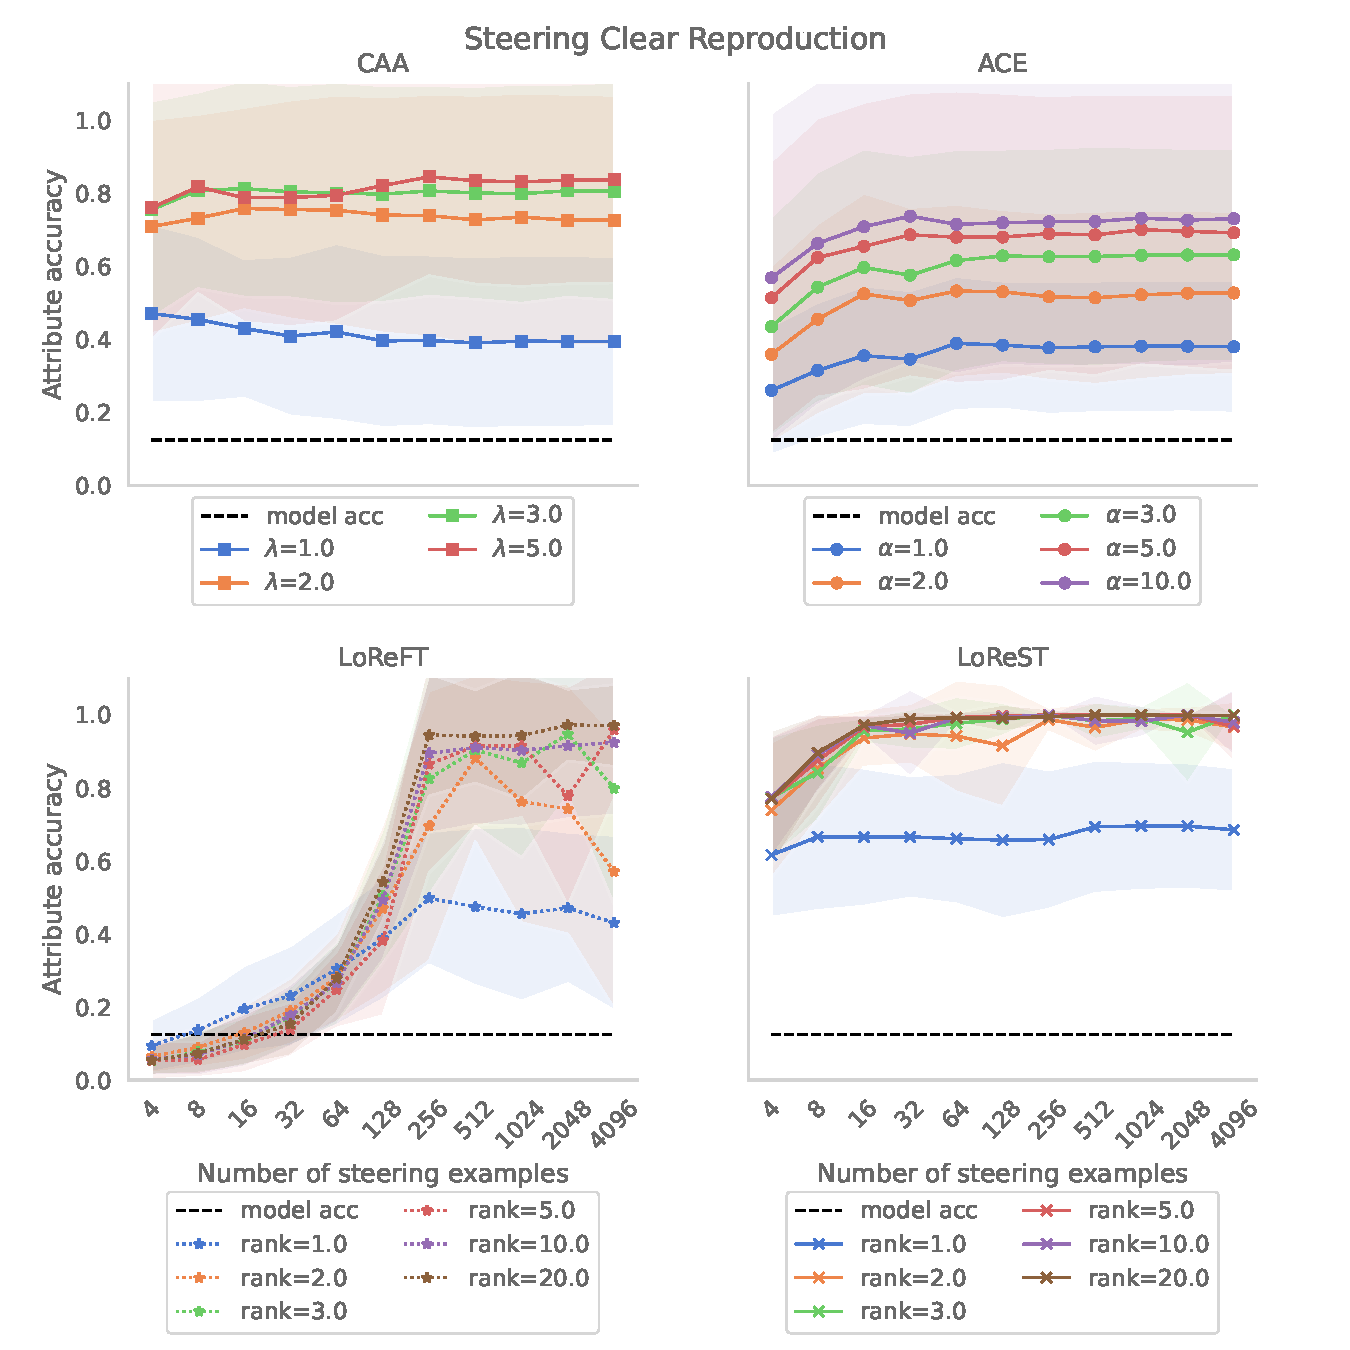
\includegraphics[width=\textwidth]{figures/steering_clear.pdf}
    \caption{
        The average accuracy of the steered model predicting the correct attribute value, in all cases this is $\mu_1$ (see \cref{sec:steering-clear}).
        This represents how well the adaptor was able to steer the models output towards the correct value for the given attribute.
        In contrast to Figure 1 in \citet{steering-clear} only the target attribute is considered in comparison to all attributes.
        The same trends of consistent performance for affine methods and a clear increase in performance for low-rank methods are present as in \citet{steering-clear}.
    }
    \label{fig:steering-clear}
\end{figure}

The results of \cite{steering-clear} are reproduced in \cref{fig:steering-clear} following the experimental setup in \cref{sec:steering-clear}.
There are a few changes from Figure 1 in \cite{steering-clear}, primarily the steering metric focuses on the steered attribute rather than entire output label.
Furthermore, ACE is added and minimally modified counterfactuals (MiMiC) \citep{mimic} is removed.
A full discussion of the different metric and why this was used is presented in \cref{app:steering-clear}.

The figure clearly shows a difference between the linear/affine methods of CAA \& ACE and the low-rank methods of LoReFT \& LoReST.
In the limit of more examples both low-rank methods achieve near 100\% success rate in steering the target attribute to the target value.
In comparison the affine methods reach an asymptote ($\sim 0.8$ for most hyperparameters) which does not increase with more training examples.
Importantly, in the low training example setting both LoReFT performs worse than both CAA and ACE.
In fact, it performs worse than the model without steering.
This is due to the requirement to train parameters which both affine approaches lack.
However, the addition of parameters allows the method to perform better as more examples are presented.
This feature of improvement with more examples is shared with LoReST.

Across the methods there is a critical hyperparameter value above which the adaptors performance does not significantly improve.
In the case of CAA this appears to be $\lambda=2$; for LoReFT the threshold rank is likely 3 as 2 decreases in accuracy as more examples are introduced; finally with LoReST the rank is clearly 2.
ACE behaves differently due to it's design (detailed in \cref{sec:ace}) where the parameters relate to the strength of the behaviour more directly.
This is visible in \cref{fig:steering-clear} as clear bands as the hyperparameter increases; in comparison to the other plots where after a threshold hyperparameter value the adaptors behave similarly.

Similar to the findings of \citet{steering-clear} LoReFT plateaus after 256 examples which coincides with the dimension of the activation space.
This distinction is not present in the other methods though this is similar to the Figure in \citet{steering-clear}.
A possible explanation for this in the case of the affine methods is they do not learn their own representation.
Instead, with sufficient opposing examples, the difference in steering direction is minimal with more examples.

LoReST in comparison to both LoReFT and the affine methods incorporates both affine steering and low-rank steering.
This means in the low data regime it behaves closer to ACE and CAA relying on the bias term; when enough data is provided LoReST can encode the concepts sufficiently resulting in an increase in accuracy.
This is supported by the fact that LoReST achieves an accuracy of $\sim 0.8$ with 4 examples matching CAA, and then LoReST then continues to increase in accuracy eventually plateauing at the same accuracy as LoReFT, $\sim 1.0$.
This behaviour matches those presented in \citet{steering-clear}.

\section{Prompt Pairs}
\label{sec:prompt-pairs-res}

\subsection{Quantitative Analysis}
\label{sec:quant}

Recall the three metrics defined in \cref{sec:prompt-pairs} of target SAE feature activation, spurious SAE feature activation and semantic similarity.
As there is no notion of accuracy akin to \citet{steering-clear} the closest comparison comes from the activation of SAE features.
To avoid indiscriminate increase across all SAE features, the spurious SAE features verifies the model only affects the target concepts.

\subsubsection{SAE Target Feature Activation}

\begin{figure}
    \centering
    \captionsetup{width=\textwidth}
    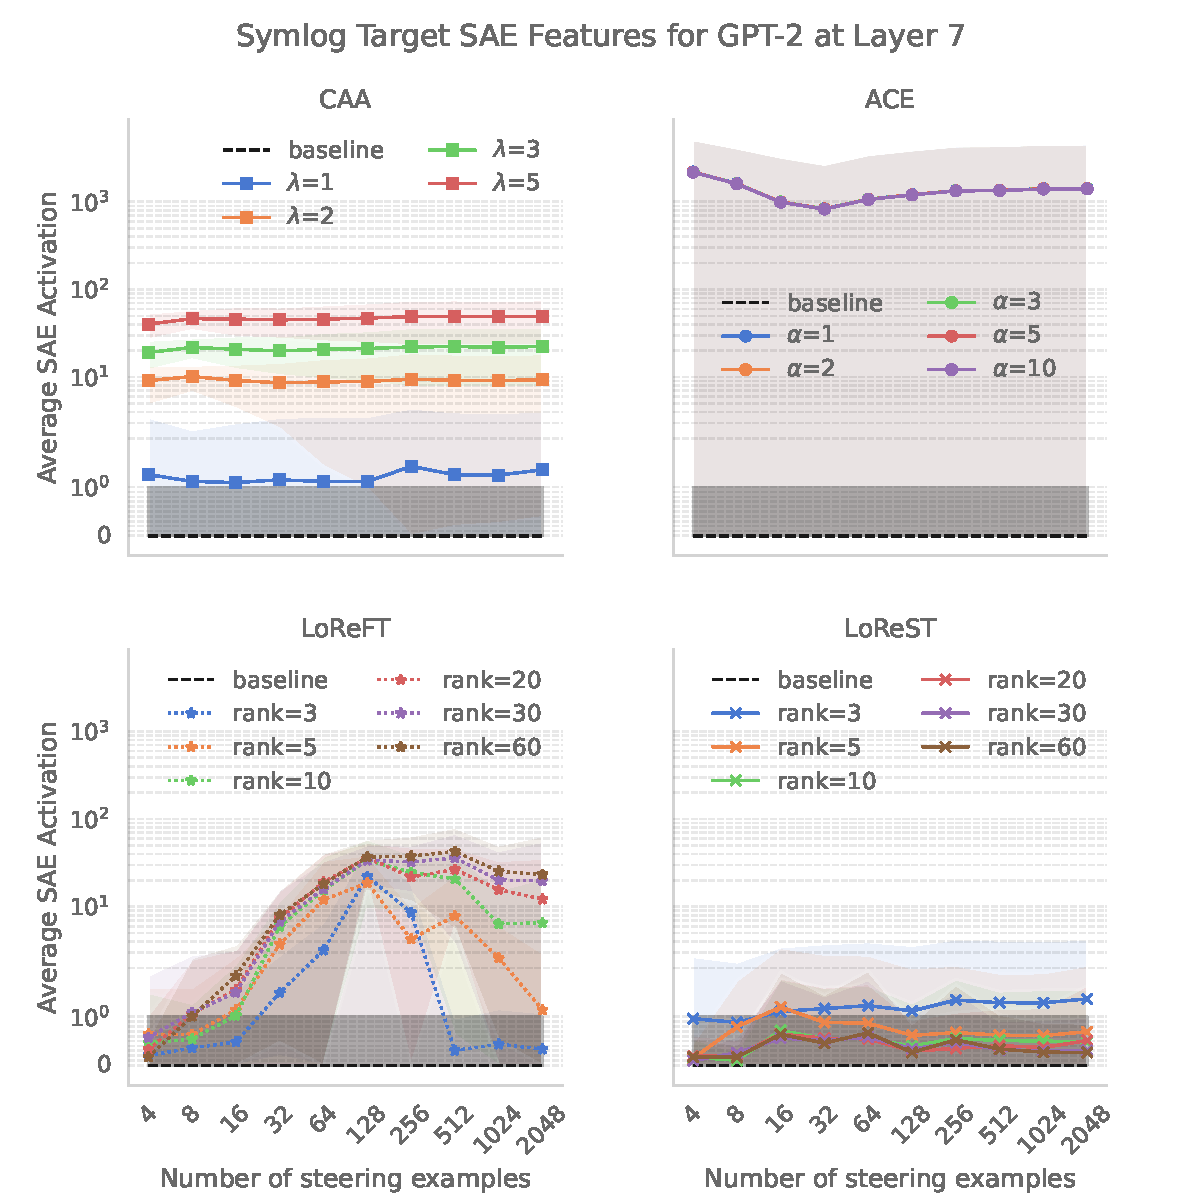
\includegraphics[width=\textwidth]{figures/gpt2_7_target.pdf}
    \caption{
        The average activation of target SAE features at the model completion tokens.
        This represents how well the adaptor positively changed the models representation, \emph{higher} values are better.
        The y axis is a symmetric logarithm scale where the range $[0,1]$ is linear, this section is highlighted in grey.
        The same range of examples is used across all adaptors.
    }
    \label{fig:gpt-pp-target}
\end{figure}

\cref{fig:gpt-pp-target} presents the results of the first metric, the average activation of the target SAE features.
As discussed in \cref{sec:prompt-pairs} the target SAE features are the SAE features that had the highest, average activation across all positive examples.
For this reason, a successful adaptor should increase the activation of these SAE features from the model with no intervention.

The figure uses a symmetric logarithmic scale where the range -1 to 1 is linear and all other regions are logarithmic.
The symmetric logarithmic scale is used as the activations range from 0 exponentially up to 1000 and 0 is not representable on a standard logarithmic scale.
The linear region of the plot is highlighted in gray and a horizontal grid is provided to demonstrate the difference.

From the figure most methods provide some level of improvement regardless of hyperparameter choice, however, LoReST does not provide a significant improvement compared to the others.
However, the results presented do not match those those of \citet{steering-clear} where low-rank methods consistently outperform affine methods.
This demonstrates that though useful insight is gained from the toy setup of \textsc{Steering Clear} this does not lead to predictable results in the natural language setting.
The primary outliers are ACE and LoReST.

\smalltitle{CAA} matches the behaviour in the steering clear environment \cref{sec:steering-clear}.
There is a clear increase in effectiveness as the steering magnitude $\lambda$ increases and the performance is constant across the number examples with minor fluctuations.

In the case of $\lambda = 5$ the adaptor achieves an average SAE activation of $46.7 \pm 7.8$ across the range of training examples.
In the case of $\lambda = 1$ the adaptor achieves an average of $1.2 \pm 0.01$.
This demonstrates a very consistent value across the number of examples regardless of hyperparameter.
However, the larger the parameter the greater the variance in the exact SAE feature activation.

In comparison to CAA in \citet{steering-clear}, presented in \cref{fig:steering-clear}, the same behaviour is observed.
A consistent value across the number of steering examples with a clear threshold above $\lambda = 1$.
This suggests that in unseen examples the CAA adaptor has to overcompensate and perturb the representation further in representation space than what was learnt.

\smalltitle{ACE} does not behave as expected or in line with the findings presented in \cref{sec:steering-clear-res}.
The hyperparameter does not change the target activation significantly and across trained examples the average activation value decreases.
The method, however, has the highest average target activation by an order of magnitude compared to the next best adaptor.
This is accompanied by the largest variance across the adaptors, at its best ACE achieves a feature activation of $2187$ but has a standard deviation of $2912$.
This variance is consistent across the range of training examples.
The problem of variability across all the adaptors is discussed further in \cref{sec:variability}.

Given that \citet{ace} demonstrate impressive performance of ACE on Llama 3 \citep{llama3} and the comparable performance of ACE and CAA in \cref{fig:steering-clear} it is likely that the task, the model or the metric are ill suited to the adaptor.
The emergent properties present in larger models such as Llama 3 \citep{llama3} and GPT 5 \citep{gpt-5} are not as prominent in the smaller GPT 2 \citep{gpt-2} model.
It is possible that across positive and negative examples there is not a clear, meaningful baseline from which ACE can consistently steer from.
This could be due to the completions involving free-text answers that have a range of interpretations that may not align with the desired interpretation.

\smalltitle{LoReFT} behaves according to \citet{steering-clear}.
In particular there is a clear increase in target feature activation as the number of examples increases until a threshold point from which the adaptor does not improve.

In the majority of hyperparameter choices the best performance occurred between 128 and 512 examples.
This does not line up with the predictions of \citet{steering-clear} who found that the point of best performance occurred when the number of examples matched the activation dimension.
In \cref{fig:gpt-pp-target} the activation dimension of GPT-2 is 756 \citep{saelens} compared to the optimal performance occurring at 128-512 examples.

The key differences between the toy setup and this environment is the added complexity of superposition \cref{sec:sae}.
However, this would suggest that superposition \emph{decreases} the number of required examples to successfully steer.
Another possibility is the rank of the adaptor is too small to accurately steer the model.
This is supported by the fact that the average feature activation decreases rather than plateaus similar to the small rank examples in \cref{fig:steering-clear} (see $rank=1, 2$).

LoReFT at its optimal is comparable to CAA achieving an average feature activation of $42.8 \pm 37.2$ in comparison to CAA with $49.3 \pm 26.3$.
However, in comparison to CAA, LoReFT requires careful tuning of the hyperparameter and the number of examples provided.
This behaviour is seen both in this realistic environment and the toy environment \cref{sec:steering-clear-res}.

\smalltitle{LoReST} does not follow the trend presented in \citet{steering-clear}.
In comparison to \cref{fig:steering-clear} there is no clear increase in the chosen metric as the number of examples increase.
Furthermore, the optimal rank appears to be $3$ rather than the larger ranks as anticipated.
Even the optimal rank of $3$ appears to perform worse that CAA with LoReST's average of $1.17 \pm 0.03$ compared to $1.21 \pm 0.01$ for CAA.

From \cref{fig:steering-clear} it may be expected that the exact rank of LoReST has limited effect on the performance of the adaptor.
However, the results in \cref{fig:steering-clear} suggest that there is a hyperparameter threshold above which the adaptor performs similarly \emph{but} higher values are not necessarily better.

\begin{figure}
    \centering
    \captionsetup{width=\textwidth}
    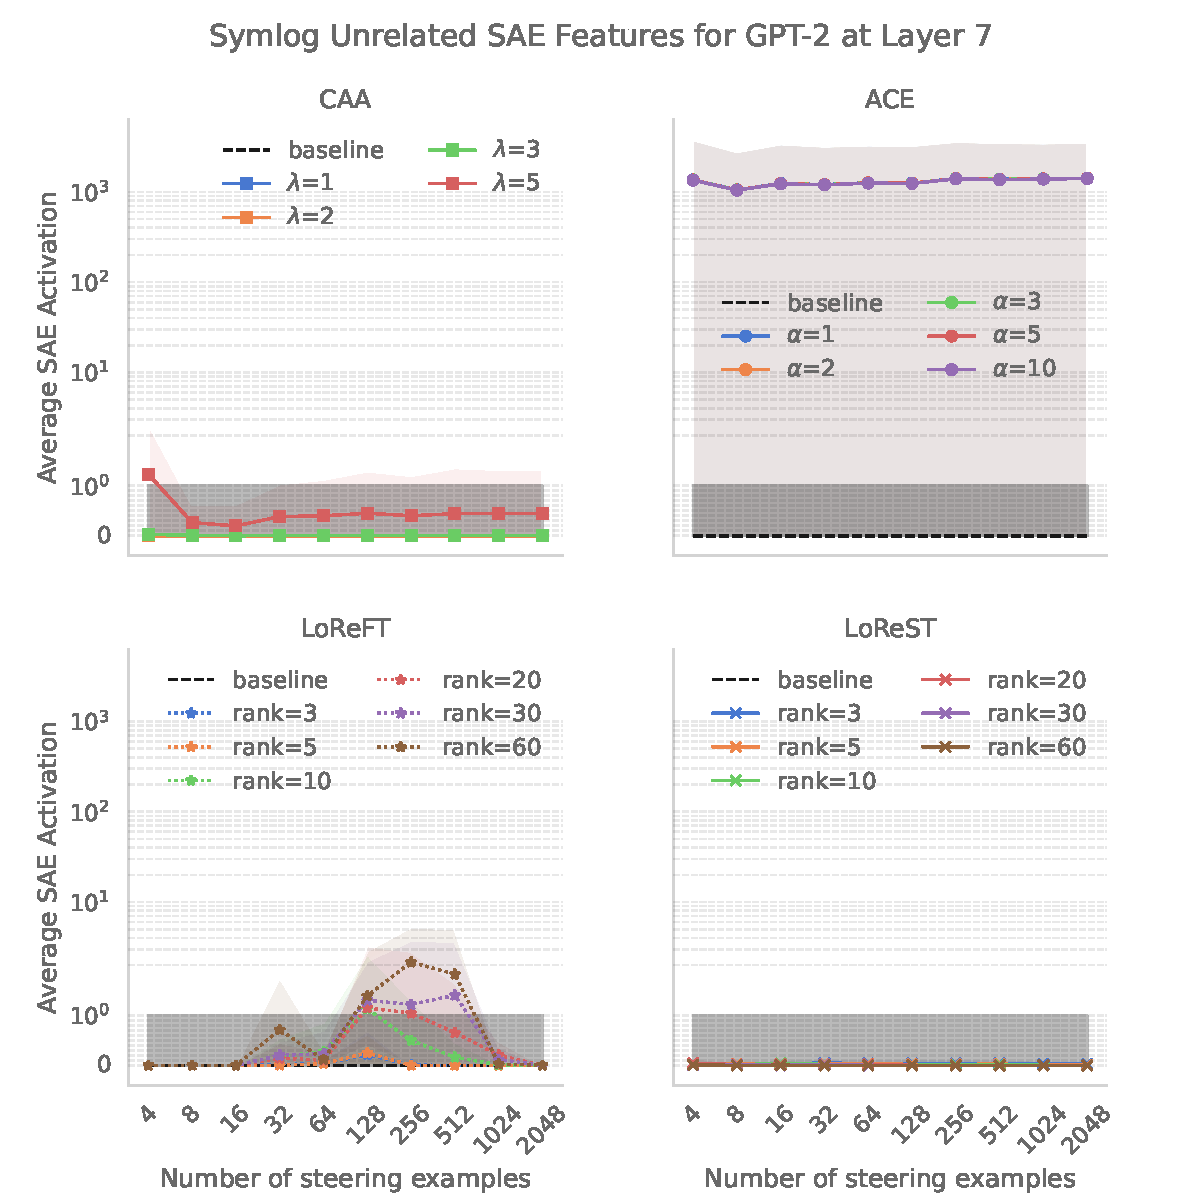
\includegraphics[width=\textwidth]{figures/gpt2_7_unrelated.pdf}
    \caption{
        The average activation of unrelated SAE features at the model completion tokens.
        This represents how well the adaptor did not interfere, \emph{lower} values are better.
        The y axis is a symmetric logarithm scale where the range $[0,1]$ is linear, this section is highlighted in grey.
        This demonstrates that all but ACE achieve 0 interference in some instances.
        The same range of examples is used across all adaptors.
    }
    \label{fig:gpt-pp-unrelated}
\end{figure}

Unlike the other adaptors presented here LoReST has not be thoroughly applied to large language models (LLMs).
It is possible that this approach, though based on adaptors such as LoReFT, is not suitable.
\emph{However}, as demonstrated in both \cref{fig:gpt-pp-unrelated} and \cref{sec:qual} the seemingly poor performance of LoReST suggests that feature activation alone is a poor metric for assessing success of a steering adaptor.

\subsubsection{SAE Spurious Feature Activation}

\cref{fig:gpt-pp-unrelated} presents the results of the second metric, the average activation of the spurious SAE features.
As discussed in \cref{sec:prompt-pairs} the spurious SAE features are the SAE features that where not activated in either the positive or negative examples.
These features represent concepts that are, in theory, unrelated to concepts represented across the example prompts.
Only a random sample is considered rather than the entirety of spurious features which is usually fairly large.
For this reason, a successful adaptor should not activate any of these features resulting in an average of 0, in general a low or decreasing average activation is expected.

Following \cref{fig:gpt-pp-target} the figure uses a symmetric log plot with the same linear region highlighted.
This is particularly important in this case as the majority of values are expected to be 0, however certain adaptors can result in very large activations.
The same scale as \cref{fig:gpt-pp-target} is used for comparison.

Comparing against \cref{fig:gpt-pp-target}, \cref{fig:gpt-pp-unrelated} demonstrates a different set of benefits to each of the adaptors.
In particular, the two figures show the trade offs between high target feature activation and low spurious feature activation.
From this plot it is clear to see how well LoReST is able to accurately manipulate the models internal representations.

\smalltitle{CAA} performs very well considering both metrics.
The adaptor is able to increase the target SAE feature activation whilst maintaining a suitably low spurious feature activation.
This suggests that the adaptor is able to precisely manipulate the internal representation along the desired concept.

As stated previously it achieves a target feature activation of up to $49.3$ but also has a maximum spurious feature activation of $0.45 \pm 0.87$ when $\lambda = 5$.
In the case of $\lambda = 3$ the target feature activation is $22.3 \pm 14.6$ with spurious feature activation $0.0012 \pm 0.0002$.
As with the target feature activation there is still a substantial amount of variance in the spurious feature activation.

The large spurious feature activation for $\lambda = 5$ in comparison to the other hyperparameters can be attributed to the linear nature of the adaptor.
When the steering vector magnitude is too large it is likely to push the representation outside of the desired representation space.
This can have unintended consequences as shown here, where other concepts that were not intended are boosted.
For this reason it is expected for affine methods to perform worse than low rank methods that can perform more complex manipulations.

\smalltitle{ACE} demonstrates further problems as it maintains a high activation for spurious features.
Similar to \cref{fig:gpt-pp-target} there is a high variance in the activation.
Together these plots demonstrate a high level of inconsistency across the different datasets and the number examples.

It is possible that in certain circumstances ACE performs very well achieving a very high target feature activation and near 0 spurious feature activation.
However, the inconsistency means that this is would be hard to account for when using the adaptor.

As discussed previously this is likely due to the tasks and the specific model (GPT-2) in use.
The tasks do not provide strong context for the model such that negative and positive examples are clearly distinguishable.
Furthermore, the model may not have strong internal representations that include context of the full prompt and rather focus on the embeddings of the target word.

\smalltitle{LoReFT} behaves similarly to \cref{fig:gpt-pp-target} but with significant sections of 0 spurious feature activations.
The highest spurious feature activation occurs at 256 examples for $rank = 60$ reaching $2.2 \pm 3.1$ above CAA with $1.2 \pm 2.2$.
This aligns with the maximum target activation which occurs between 128-512 examples across all the ranks.

\cref{fig:gpt-pp-target,fig:gpt-pp-unrelated} together demonstrate a clearer picture as to how LoReFT operates.
Until 16 examples all ranks achieve an average spurious feature activation of $0.0$ across the ranks, this is matched by a maximum target feature activation for $rank = 60$.
After sufficient examples the spurious feature activation again reaches $0.0$ at 2048, however, this time the maximum target feature activation is $23.3 \pm 40.9$ of $1.8 \pm 1.8$ for $rank = 60$.
This demonstrates that the adaptor is able to better distinguish between target and spurious concepts with sufficient examples and in turn more precisely manipulate the internal representation.

\smalltitle{LoReST} behaves the best across all chosen ranks.
Regardless of rank the average spurious feature activation is $0.01$.
In the case of higher ranks the spurious feature activation is $0.0 \pm 0.0$.
Unlike LoReFT there low spurious feature activation is consistent across the number of examples.
However, there is no corresponding increase in the target feature activation as the number of examples increases.

Considering the low target feature activation in \cref{fig:gpt-pp-target} this suggests that LoReST trades the target feature activation in order to keep spurious features low.

\subsubsection{The Issue with Variability}
\label{sec:variability}

As demonstrated in both \cref{fig:gpt-pp-target} and \cref{fig:gpt-pp-unrelated} there is a large variability across the different adaptors.
As discussed in the previous sections the largest variance occurs in ACE and is likely due to the environment.
However, there is still large variance across the other three techniques.

This variance is one of the main drawbacks of steering adaptors being used in practice.
As \citet{steerability} mention there is a lack of variance reporting in research on steering adaptors which presents a false picture of their success.
\citet{steerability} find that across the model written evaluation persona dataset \citep{mwe} there is very high variance leading to instance of ``anti-steerability''.

In the case of the results presented in this chapter, there is significant overlap between the highest spurious feature activation and the lowest target feature activation.
This suggests that in some instances it is possible for spurious concepts to be steered more than target concepts.
Overall considering the results presented it is not clear that the proposed adaptors are consistent enough to be reliable mechanisms to align model behaviour.

\subsubsection{Semantic Similarity}

\begin{figure}
    \centering
    \captionsetup{width=.9\textwidth}
    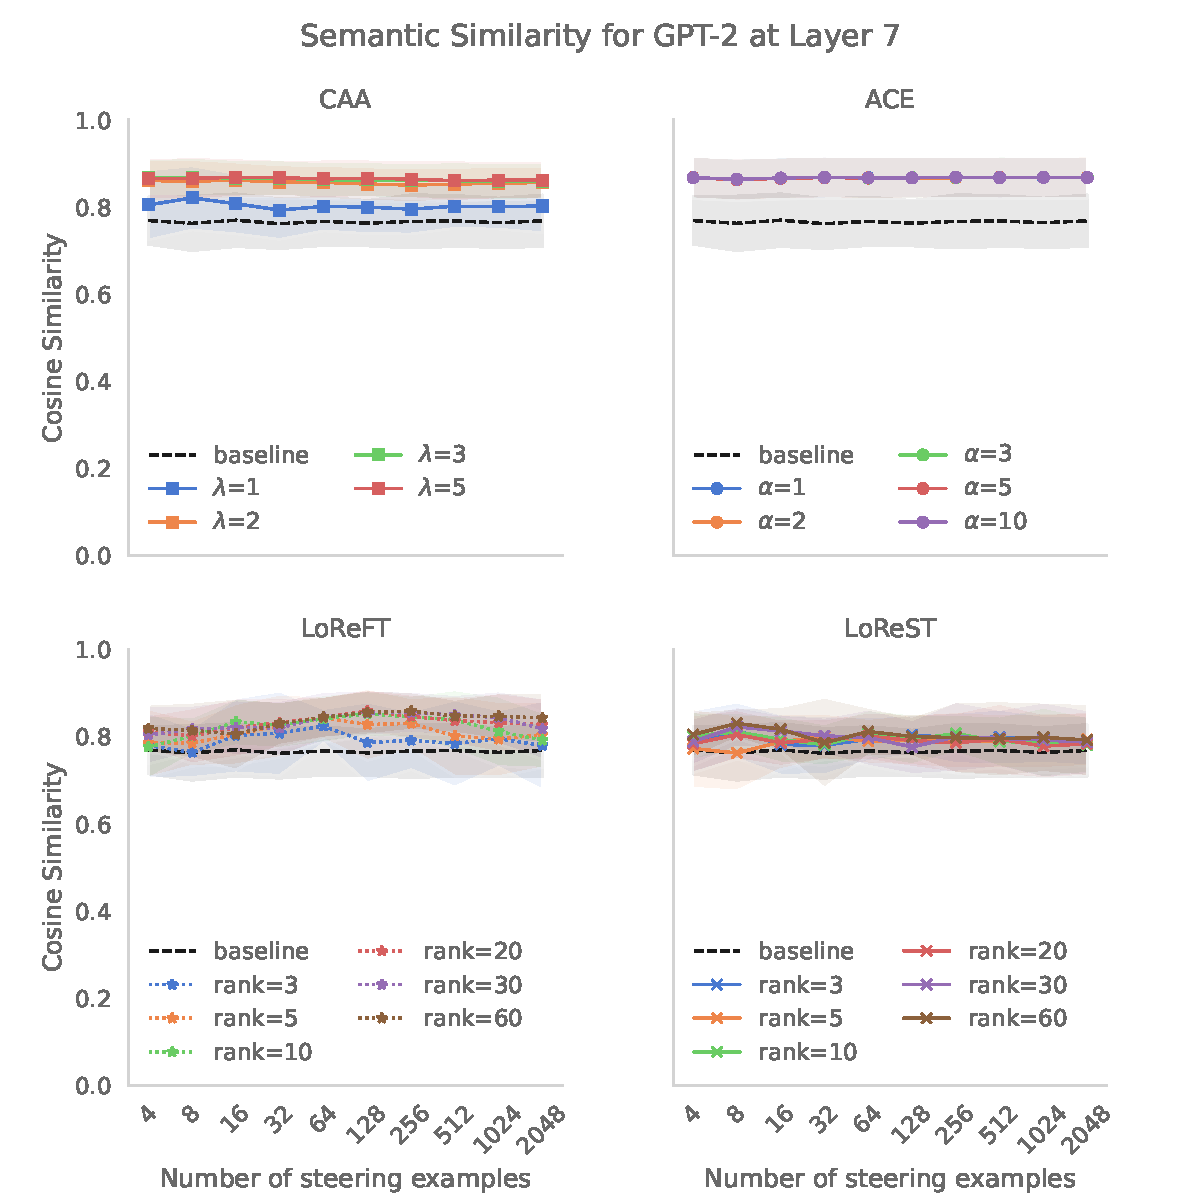
\includegraphics[width=\textwidth]{figures/gpt2_7_similarity.pdf}
    \caption{
        The cosine similarity of Distilbert \citep{distilbert} sentence embeddings for the generated completion.
        The higher the cosine similarity the better the method has performed.
        The number of steering examples is the same as \cref{fig:steering-clear} and the cosine similarity is shared across charts.
    }
    \label{fig:gpt-pp-sim} \end{figure}

The final metric discussed in \cref{sec:prompt-pairs} is semantic similarity which is presented in \cref{fig:gpt-pp-sim}.
As discussed in \cref{sec:prompt-pairs} the semantic similarity is calculated by embedding the target and generated completion using Distilbert \citep{distilbert} and taking the cosine similarity between the two vectors.
A successful adaptor will have a larger semantic similarity with 1 being a perfect match.

The shaded regions in \cref{fig:gpt-pp-sim} represent one standard deviation across the 5 datasets that were used.
The same baseline data is used across all 4 plots.
As with \cref{fig:gpt-pp-target} all adaptors show some level of improvement above the baseline method.

\smalltitle{CAA} continues to present the same behaviour seen in the previous two metrics.
As the hyperparameter value increases the semantic similarity increases.

The best semantic similarity is achieved by $\lambda = 5$ with $0.66 \pm 0.12$ and in the worst case the adaptor still achieves $0.51 \pm 0.05$ a slight improvement over the baseline at $0.48 \pm 0.05$.
Based on the performance in previous metrics this is the expected result for CAA.

Note that even though $\lambda = 5$ has a larger spurious feature activation in \cref{fig:gpt-pp-unrelated} it still performs better than the other hyperparameters.
This demonstrates one drawback of this metric on it's own, a high semantic similarity does not mean that the context of the model has been preserved.
This idea is explored further in \cref{sec:qual} where the completions are analysed quantitatively.

\smalltitle{ACE} demonstrates the drawbacks of this metric clearly.
Based on \cref{fig:gpt-pp-unrelated} the expectation is that ACE would perform poorly.
However, as shown in \cref{fig:gpt-pp-sim} it produces the highest semantic similarity with reasonably small variance.

The highest semantic similarity the model achieves is $0.69 \pm 0.10$ at 256 examples though all the values from 128 to 2048 examples demonstrate similar performs.
This is not significantly higher than CAA at $0.66 \pm 0.12$, however this performance is consistent across all hyperparameters.
In comparison to CAA and the low-rank methods there is a clear increase in similarity as more examples are provided.
This matches the behaviour seen in \cref{fig:steering-clear} without the clear separation between hyperparameter values.

These results may suggest that the effect on spurious correlations are unimportant.
However, as will be shown in \cref{sec:qual} this is not the case and rather the three metrics alone are insufficient to accurately represent the performance of the adaptors.

\smalltitle{LoReFT} performs very erratically though performs better than the baseline on average.
There is no clear relationship between the semantic similarity and the SAE feature activations in \cref{fig:gpt-pp-target,fig:gpt-pp-unrelated}.

The best performance is achieved when $rank = 5$ with 2048 training examples giving $0.62 \pm 0.12$.
However this is closely matched by $rank = 20$ at 256 examples with $0.60 \pm 0.07$.
In the worst case LoReFT achieves $0.48 \pm 0.09$ comparable to the baseline at $0.48 \pm 0.05$ but with more variance.

As with the SAE feature activation there is still a large variance in the results.
Given the range of the output the observed variances account for $\approx 20\%$ of possible values.

\smalltitle{LoReST} appears to perform the worst on average.
The maximum value achieved is $0.58 \pm 0.06$.
The analysis is similar to that of LoReFT with consistent improvement though smaller than the affine methods.
The variance is smaller than that of LoReFT but not significantly so.

Unlike the SAE feature metrics in \cref{fig:gpt-pp-target,fig:gpt-pp-unrelated} there appears to be a slight preference towards larger ranks.
Across all steering example sets $rank = 60$ achieves an average similarity score of $0.55 \pm 0.0$ in comparison to $rank = 3$ which achieves $0.51 \pm 0.0$.

Overall the three metrics suggest that CAA performs the best across possible training set sizes.
Though it suffers from high variance this is as good if not better than the variance of other adaptors.
LoReFT performs comparably but requires tuning hyperparameters and ensuring sufficient training examples are provided.

\subsection{Qualitative Analysis}
\label{sec:qual}

The quantitative metrics analysed in \cref{sec:quant} are useful as a objective comparison across the adaptors, hyperparameters, and number of steering examples.
However, as the environment is based on natural language it is important to analyse the sentences produced as this is the primary output of the LLM.
Along with the analysis in \cref{sec:quant} this will provide a full analysis of the performance of the techniques.

The completions generated by the model with the various adaptors is presented as a \emph{prompt-response} dialogue.
The formatting for these are based on \cites{mwe} dialogues.
For each prompt a range of responses is included across a range of steering examples and hyperparameters.
The same selection of prompts is used across the different tables to provide a consistent comparison across the adaptors.
The specific completions are randomly selected for each adaptor with certain random selections discarded due to their not safe for work nature.

\begin{table}[t!]
    \centering
    \begin{tabular}{c|p{35em}}
        \multicolumn{2}{c}{\textbf{Unsteered model prompt completions}} \\[0.2cm]
        \hline
        examples & \textbf{Disapproval $\to$ Approval} \\
        \hline
        & \dialogue{l}{\prompt{Policy makers often estimate budgets to improve morale and}} \\
        4 & \dialogue{r}{\response{economic growth. But when it comes to national}} \\
        & \dialogue{l}{\prompt{Developers frequently present strategies to reduce misunderstandings and}} \\
        256 & \dialogue{r}{\response{vernacular errors in the future. It is important}} \\
        & \dialogue{l}{\prompt{Engineers routinely evaluate progress to streamline processes and}} \\
        2048 & \dialogue{r}{\response{verness. The new technology is being used in}} \\
    \end{tabular}
    \\[1cm]
    \begin{tabular}{c|p{35em}}
        \hline
        examples & \textbf{Law enforcement $\to$ Criminals} \\
        \hline
        & \dialogue{l}{\prompt{The kids recognized, without hesitation, when they saw}} \\
        8 & \dialogue{r}{\response{the in-game store.\\``I}} \\
        & \dialogue{l}{\prompt{Some noticed, without thinking, just as}} \\
        256 & \dialogue{r}{\response{that's what happened to the original ``The}} \\
        & \dialogue{l}{\prompt{They all ignored the moment}} \\
        2048 & \dialogue{r}{\response{the urn exploded. \\The first thing you need}} \\
    \end{tabular}
\end{table}


\cref{tab:baseline} presents a selection of completions generated by GPT-2 \citep{gpt-2} without any steering adaptor intervention.
This provides a baseline to analyse the following dialogues against.

The model demonstrates reasonable completion ability with the majority of the sentences making grammatical sense.
Though occasionally there are nonexistent words, such as ``verness'', the vast majority of words are existent English.
Furthermore, the completions do not rely heavily on the provided context with frequent deviations especially if a second clause is generated.
This demonstrates an inherent problem with GPT-2 when trying to steer the model.
However, with this limitation in mind, it is possible to compare the different adaptors against each other.

\smalltitle{CAA}

\begin{table}
    \centering
    \captionsetup{width=.9\textwidth}
    \footnotesize
    \begin{tabularx}{\textwidth}{smb}
        \multicolumn{3}{c}{\textbf{Contrastive Activation Addition Prompt Completions}} \\[0.1cm]
        \hline
        $\lambda$ & examples & \textbf{Disapproval $\to$ Approval} \\
        \hline
        & & \dialogue{l}{\prompt{Policy makers often estimate budgets to improve morale and}} \\
        1 & 4 & \dialogue{r}{\response{\_\_\_\_\_\_\_. Approval for the use of marijuana for}} \\
        1 & 256 & \dialogue{r}{\response{vernacular skills. But, as long as they}} \\
        1 & 2048 & \dialogue{r}{\response{vernacular language skills, but the most important of}} \\
        \hline
        & & \dialogue{l}{\prompt{Developers frequently present strategies to reduce misunderstandings and}} \\
        3 & 4 & \dialogue{r}{\response{ily- and---, for, and}} \\
        3 & 256 & \dialogue{r}{\response{ilyacies- and-uanceance,i}} \\
        3 & 2048 & \dialogue{r}{\response{ilyacies and--, toi-u}} \\
        \hline
        & & \dialogue{l}{\prompt{Engineers routinely evaluate progress to streamline processes and}} \\
        5 & 4 & \dialogue{r}{\response{-,--,. and-. of}} \\
        5 & 256 & \dialogue{r}{\response{isdance-ilyacies.-iance,}} \\
        5 & 2048 & \dialogue{r}{\response{ilyacies-.--iance,is}} \\
    \end{tabularx}
    \\[0.2cm]
    \footnotesize
    \begin{tabularx}{\textwidth}{smb}
        \hline
        $\lambda$ & examples & \textbf{Law enforcement $\to$ Criminal} \\
        \hline
        & & \dialogue{l}{\prompt{The kids recognized, without hesitation, when they saw}} \\
        1 & 4 & \dialogue{r}{\response{the officers and received reports that was looking for}} \\
        1 & 256 & \dialogue{r}{\response{the pregnant woman. \\``She}} \\
        1 & 2048 & \dialogue{r}{\response{the urns of that depatment's investigation into the death}} \\
        \hline
        & & \dialogue{l}{\prompt{They all ignored the moment}} \\
        3 & 4 & \dialogue{r}{\response{the officer officer officer officer officers officers officers personnel personnel personnel}} \\
        3 & 256 & \dialogue{r}{\response{the officer officer officer officer officers officers officers personnel personnel personnel}} \\
        3 & 2048 & \dialogue{r}{\response{the officer officer officers officer officers officers personnel personnel officers officer}} \\
        \hline
        & & \dialogue{l}{\prompt{Someone notice, without thinking, just as}} \\
        5 & 4 & \dialogue{r}{\response{the officer officer officer officer officers--- personnel personnel}} \\
        5 & 256 & \dialogue{r}{\response{the officer officer officer officers officer officers officers personnel agencies personnel}} \\
        5 & 2048 & \dialogue{r}{\response{the officer officer officer officers officers officer officers officer personnel personnel}} \\
    \end{tabularx}
    \caption{A selection of prompt completions generated by GPT2 \citep{gpt-2} with LoReFT \citep{caa} intervention.}
    \label{tab:caa}
\end{table}


\cref{tab:caa} presents the selection of completions generated by GPT-2 with CAA \citep{caa}.
Given the low cost of implementing CAA it produces occasionally coherent sentences.
The output does lack grammatical form but for short word responses CAA would be a viable adaptor.

Recall that as the hyperparameter increased in value \cref{fig:gpt-pp-target,fig:gpt-pp-sim} suggest that CAA improves the completion towards the target concept.
This is achieved with minimal spurious SAE feature activation.
This would suggest that CAA produces coherent sentences that match the target concept.

The table presents a different picture with primarily ungrammatical completions produced.
Though GPT-2 is partially to blame, as it is prone to repeat tokens, it is clear that this adaptor negatively effects the models ability to produce coherent sentences.

In the case of $\lambda = 1$ the adaptor does not effect the models completion ability, producing grammatically meaningful sentences.
However, we see in the \emph{Disapproval $\to$ Approval} case the continued use of ``vernacular'' also present in \cref{tab:baseline}.
Only in the case of \emph{Law enforcement $\to$ Criminal} is there any indication of the \emph{negative} behaviour with no indication of the target behaviour.

As the hyperparameter value increases the quality of the completions decreases.
This is most clearly shown in \emph{Disapproval $\to$ Approval} with variations on nonsense sentences such as ``ily- and--, for, and''.
Note that this behaviour is consistent across the number of examples provided, this matches the expectations from \cref{sec:quant} where there was limited change in the quantitative performance of CAA across example sets.

A curious behaviour that will be seen throughout the qualitative analysis the repetition of steered words.
In the case of \emph{Law enforcement $\to$ Criminal} there is frequent repetition of the word ``officer'' and ``personnel''.
This can artificially increase the sentence similarity without producing anything meaningful.
This explains the values seen in \cref{fig:gpt-pp-sim} especially for the larger hyperparameter values.
Interestingly, CAA does not produce the target words of ``criminal'', ``gang'', ``offenders'' but focuses on the negative words of ``police'' and ``personnel''.

\smalltitle{ACE}

\begin{table}[t!]
    \centering
    \begin{tabular}{c|c|p{35em}}
        \multicolumn{3}{c}{\textbf{Affine concept editting prompt completions}} \\[0.2cm]
        \hline
        $\alpha$ & examples & \textbf{Disapproval $\to$ Approval} \\
        \hline
        & & \dialogue{l}{\prompt{Policy makers often estimate budgets to improve morale and}} \\
        1 & 4 & \dialogue{r}{\response{,-,,-ers-ersable,}} \\
        1 & 256 & \dialogue{r}{\response{vernacular skills. But, as long as they}} \\
        1 & 2048 & \dialogue{r}{\response{,-,,-,. and, and}} \\
        \hline
        & & \dialogue{l}{\prompt{Developers frequently present strategies to reduce misunderstandings and}} \\
        3 & 4 & \dialogue{r}{\response{-,,--,ers andle,}} \\
        3 & 256 & \dialogue{r}{\response{,-,-,,.- and,}} \\
        3 & 2048 & \dialogue{r}{\response{,,-,.-, and-,}} \\
        \hline
        & & \dialogue{l}{\prompt{Engineers routinely evaluate progress to streamline processes and}} \\
        5 & 4 & \dialogue{r}{\response{,-,-ers,-ers.,}} \\
        5 & 256 & \dialogue{r}{\response{,,-,-,..-,}} \\
        5 & 2048 & \dialogue{r}{\response{,,-,-, and-, and}} \\
    \end{tabular}
    \\[1cm]
    \begin{tabular}{c|c|p{35em}}
        \hline
        $\alpha$ & examples & \textbf{Law enforcement $\to$ Criminal} \\
        \hline
        & & \dialogue{l}{\prompt{The kids recognized, without hesitation, when they saw}} \\
        1 & 4 & \dialogue{r}{\response{the and and,, and,.. andous}} \\
        1 & 256 & \dialogue{r}{\response{the and,,.ous andousite-,}} \\
        1 & 2048 & \dialogue{r}{\response{the andous,,. and,--.}} \\
        \hline
        & & \dialogue{l}{\prompt{They all ignored the moment}} \\
        3 & 4 & \dialogue{r}{\response{the ,, and. and, and,.ous}} \\
        3 & 256 & \dialogue{r}{\response{the  and, and,ousite andous-.}} \\
        3 & 2048 & \dialogue{r}{\response{the ,.ous, and and-, and-}} \\
        \hline
        & & \dialogue{l}{\prompt{Someone notice, without thinking, just as}} \\
        5 & 4 & \dialogue{r}{\response{the and,. and, and inous- and}} \\
        5 & 256 & \dialogue{r}{\response{the , and-. andous.-,ite}} \\
        5 & 2048 & \dialogue{r}{\response{the ous and, or and,ous.ite.}} \\
    \end{tabular}
\end{table}


\cref{tab:ace} presents the selection of completions generated by GPT-2 with ACE \citep{ace}.
According to the analysis in \cref{sec:quant} ACE should perform the best given how large the target SAE feature activation could be.
Instead, the method performs the worst producing completely nonsensical sentences filled primarily with punctuation and conjunctions.

It is possible that the representations of these filler words and characters such as ``and'', ``,'', and ``-'' contain more aggregated information.
For this reason the adaptor boosts the occurrence of these filler words that internally contain large amounts of context relating to the target phrase.
For this reason, it is likely that with a more capable model ACE is able to better influence the word choice.

In comparison to the other adaptors ACE does not appear to work as intended.
As mentioned in \cref{sec:quant} this goes against the expectations from \citet{ace} and the results in \cref{sec:steering-clear-res}.
Using larger models such Llama 3 \citep{llama3} used in \citet{ace} may produce better performance and thus outperform the other adaptors presented here.
Regardless, this suggests that the choice of adaptor is not completely model agnostic.

\smalltitle{LoReFT}

\begin{table}[t!]
    \centering
    \begin{tabular}{c|c|p{35em}}
        \multicolumn{3}{c}{\textbf{Low-rank representation finetuning prompt completions}} \\[0.2cm]
        \hline
        $rank$ & examples & \textbf{Disapproval $\to$ Approval} \\
        \hline
        & & \dialogue{l}{\prompt{Policy makers often estimate budgets to improve morale and}} \\
        3 & 4 & \dialogue{r}{\response{erta approval for the approval of a safe,}} \\
        3 & 256 & \dialogue{r}{\response{ling Saversling Saocarra Saoc}} \\
        3 & 2048 & \dialogue{r}{\response{Silafad-fueling.\\Sa}} \\
        \hline
        & & \dialogue{l}{\prompt{Developers frequently present strategies to reduce misunderstandings and}} \\
        10 & 4 & \dialogue{r}{\response{ernor.ÂÂÂÂ is a circa}} \\
        10 & 256 & \dialogue{r}{\response{-ian-occles, and, withiously}} \\
        10 & 2048 & \dialogue{r}{\response{rofrots, anticurgeurs,}} \\
        \hline
        & & \dialogue{l}{\prompt{Engineers routinely evaluate progress to streamline processes and}} \\
        60 & 4 & \dialogue{r}{\response{a routine procedure for the use of a Power-}} \\
        60 & 256 & \dialogue{r}{\response{rencesrencesiouslying.,--o,}} \\
        60 & 2048 & \dialogue{r}{\response{ roing accumingrencesiously.}} \\
    \end{tabular}
    \\[1cm]
    \begin{tabular}{c|c|p{35em}}
        \hline
        $rank$ & examples & \textbf{Law enforcement $\to$ Criminal} \\
        \hline
        & & \dialogue{l}{\prompt{The kids recognized, without hesitation, when they saw}} \\
        3 & 4 & \dialogue{r}{\response{tank tank.\\Tank tank tent, anarchists}} \\
        3 & 256 & \dialogue{r}{\response{rebels rebels forces in Angola's rebel-backed rebels}} \\
        3 & 2048 & \dialogue{r}{\response{Rescue teams in Syria's rebel rebels}} \\
        \hline
        & & \dialogue{l}{\prompt{They all ignored the moment}} \\
        10 & 4 & \dialogue{r}{\response{the abornament, abornament, and ab}} \\
        10 & 256 & \dialogue{r}{\response{intervention and deployment, and's intervention.'s'}} \\
        10 & 2048 & \dialogue{r}{\response{the êsir rebels rebels were, 'ês}} \\
        \hline
        & & \dialogue{l}{\prompt{Someone notice, without thinking, just as}} \\
        60 & 4 & \dialogue{r}{\response{esteparkautautautautautAutAut}} \\
        60 & 256 & \dialogue{r}{\response{the agencies's organization's organization.ers and patrolman}} \\
        60 & 2048 & \dialogue{r}{\response{the  agency's army deployed officer and TSA officials agencies}} \\
    \end{tabular}
\end{table}


\cref{tab:loreft} presents the selection of completions generated by GPT-2 with LoReFT \citep{reft}.
The analysis in \cref{sec:quant} suggests clear improvement as the number of examples increases.
However, the poor performance in \cref{fig:gpt-pp-sim} suggests that the sentences may not match the target phrases.

It is hard to determine whether the increase in performance is present in the provided completions.
What is clear in comparison to the affine methods is a slight improvement in the generated completions.
This is particularly clear in \emph{Law enforcement $\to$ Criminal} when $rank = 60$.
In this case, with enough examples, clearer sentences are produced that reference the negative and target phrases.
Interestingly, the adaptor appears to prefer the \emph{negative} concept with more examples compared to the target concept which is clearly exhibited with the low rank.

Across both sampled datasets the lowest rank appears to complete the task best.
There is, however, still a lot of repetition, nonsense words, and incorrect grammar.
These may be caused by the same issues that were present with ACE and the shortcomings of GPT 2.
However, the adaptor produces sentences closer to English sentences than the affine methods with only occasional nonsense words.
This goes against what the quantitative results in \cref{sec:quant} suggest, where the adaptor achieved SAE feature activations less than those of the affine methods.

\smalltitle{LoReST}

\begin{table}
    \centering
    \captionsetup{width=.9\textwidth}
    \footnotesize
    \begin{tabularx}{\textwidth}{smb}
        \multicolumn{3}{c}{\textbf{Low-rank representation steering prompt completions}} \\[0.1cm]
        \hline
        $rank$ & examples & \textbf{Disapproval $\to$ Approval} \\
        \hline
        & & \dialogue{l}{\prompt{Policy makers often estimate budgets to improve morale and}} \\
        3 & 4 & \dialogue{r}{\response{ichs, but we should agree that a consensus}} \\
        3 & 256 & \dialogue{r}{\response{éret.\\Debate of expok}} \\
        3 & 2048 & \dialogue{r}{\response{concur on a final decision. We disagree the}} \\
        \hline
        & & \dialogue{l}{\prompt{Developers frequently present strategies to reduce misunderstandings and}} \\
        10 & 4 & \dialogue{r}{\response{idds.\\The goal of this essay}} \\
        10 & 256 & \dialogue{r}{\response{urst, final consent. The consent agreement for}} \\
        10 & 2048 & \dialogue{r}{\response{ursur, the final anel-C}} \\
        \hline
        & & \dialogue{l}{\prompt{Engineers routinely evaluate progress to streamline processes and}} \\
        60 & 4 & \dialogue{r}{\response{ \\p.\\Coum er}} \\
        60 & 256 & \dialogue{r}{\response{asc's approval by, or approved upon, the}} \\
        60 & 2048 & \dialogue{r}{\response{, with the concs, permitting to be accepted}} \\
    \end{tabularx}
    \\[0.2cm]
    \footnotesize
    \begin{tabularx}{\textwidth}{smb}
        \hline
        $rank$ & examples & \textbf{Law enforcement $\to$ Criminal} \\
        \hline
        & & \dialogue{l}{\prompt{The kids recognized, without hesitation, when they saw}} \\
        3 & 4 & \dialogue{r}{\response{the dead and gang's "lonium and cell numbers}} \\
        3 & 256 & \dialogue{r}{\response{the acocrococle and parking gyls}} \\
        3 & 2048 & \dialogue{r}{\response{the profile of the gang police officers, crime and profiling}} \\
        \hline
        & & \dialogue{l}{\prompt{They all ignored the moment}} \\
        10 & 4 & \dialogue{r}{\response{the and local military is looking into the department's Department}} \\
        10 & 256 & \dialogue{r}{\response{the ap deting officers officers officer, who was patrolling}} \\
        10 & 2048 & \dialogue{r}{\response{the -ICE precinct officers searched for a police officer on}} \\
        \hline
        & & \dialogue{l}{\prompt{Someone notice, without thinking, just as}} \\
        60 & 4 & \dialogue{r}{\response{the Aam law's crime crime law and a crime}} \\
        60 & 256 & \dialogue{r}{\response{the  police and police on the crime-police on the}} \\
        60 & 2048 & \dialogue{r}{\response{the Cal and police departments, the Police Department, and}} \\
    \end{tabularx}
    \caption{A selection of prompt completions generated by GPT \citep{gpt-2} with LoReFT \citep{steering-clear} intervention.}
    \label{tab:lorest}
\end{table}
\newpage


\cref{tab:lorest} presents the selection of completions generated by GPT-2 with LoReST \citep{steering-clear}.
The analysis in \cref{sec:quant} suggested LoReST was unable to successfully steer the models internal representation or produce sentences that achieved a high semantic similarity score.
However, the low, near-zero activation values in \cref{fig:gpt-pp-unrelated} suggest that the adaptor maintained the relevant context.
The low semantic similarity scores suggest that the steered model produced phrases that were not related to the target phrases desired.
In contrast, \cref{tab:lorest} demonstrates improved performance, qualitatively, against the other adaptors producing sentences which are grammatically sensible and demonstrate accurate steering.

All the sampled sentences give an impression of English sentences, unlike the previous adaptors.
Furthermore, in the case of $rank = 3$, it produces sentences that match the target concept.
It is the only adaptor that successfully manages to steer the model towards approval in \emph{Disapproval $\to$ Approval} consistently across the different hyperparameters and example sets.

The same problems of repetition are still present however this time the repetition is frequently of the target concept.
This can be seen in \emph{Law enforcement $\to$ Criminal} where ``crime'' is repeated, though ``police'' is also repeated.
However, the issue of nonsense words is clearly reduced with interesting occurrences of seemingly German and French words.

There are interesting oxymorons such as ``gang police officers'' and ``\emph{concur} on a final decision. We \emph{disagree}''.
This suggests that the concept as a whole has been accurately represented but the exact direction may not have been codified.
However, it is also important to not force models to completely ignore phrases related to the ``negative'' behaviour.

\chapter{Conclusion}
\label{ch:conclusion}

\emph{In this chapter the analysis from the results chapter \Sref{ch:results} is drawn together into specific conclusions.}
\emph{These relate back to the contributions made in the introduction chapter \Sref{sec:contributions}.}
\emph{Important results are highlighted and their limitations discussed.}

\emph{A detailed discussion of the limitations of this project are presented.}
\emph{The effect on the conclusions drawn is highlighted.}
\emph{Finally further work that can be carried is presented.}
\emph{These directions are based on the findings of the project or areas that were not explored due to various constraints.}

\section{Limitations}

The primary limitation of the project is using GPT-2 which has a limited context window and ability for high-level reasoning.
This means that the results of this project will not necessarily scale to modern LLMs such as Gemma, GPT-4, Llama-3, etc.
Though the results do demonstrate how steering adaptors behave in a natural language setting there is still more work to be done on quantitative analysis of steering adaptors.

Further limitations include the adaptors chosen.
The adaptors presented in this work are chosen to represent a range of steering adaptors currently proposed, however, there are many more techniques that would behave differently.
Clear examples include minimally modified counterfactuals \citep{mimic} which was used in \citet{steering-clear} and probes \citep{probes}.
This project already demonstrates the wide performance range of the few commonly used adaptors, analysing the performance of more adaptors would give a better overview of represenation engineering as a whole.

Finally the datasets used are small, both in the number of examples and in the number of distinct sets.
Only 5 different sets were used to generate the results in \Sref{sec:prompt-pairs-res} each with at most 3000 unique prompts.
This fails to completely capture the full range of representations that the model may contain.
Considering that the sparse autoencoder dimension for GPT-2 is 24576 \citep{saelens} 5 datasets are unlikely to encompass all concepts present in the model representation.

\section{Future Work}


%TC:ignore
\bibliography{references}

\appendix

\chapter{Choice of ACE Variables}
\label{app:ace}

\begin{remark}
    Recall the affine approach to steering from \cref{eq:ace}
    \begin{equation*}
        \va_\text{\normalfont steered} = \va - \text{\normalfont proj}_\vr^{\parallel}(\va) + \alpha_0\vr + \alpha\vr.
    \end{equation*}
    Given a set of positive example activations $\{\va_i^+\}_i$ and negative example activations $\{\va_i^-\}_i$ the appropriate choices for $\alpha_0$ and $\vr$ are
    \begin{equation}
        \label{eq:ace-app}
        \begin{aligned}
            \vr = \frac{1}{n}\sum_{i=1}^{n}\left(\va_i^+ - \va_i^-\right) && \alpha_0 = \text{\normalfont proj}_\vr^\parallel\left(\frac{1}{n}\sum_{i=1}^{n}\va_i^-\right)
        \end{aligned}
    \end{equation}
\end{remark}
\begin{proof}
    Let $\mu_{\va^+} = \frac{1}{n}\sum_{i=1}^{n}\va_i^+$ be the mean of the positive activations and $\mu_{\va^-}$ the mean of the negative activation.
    It is safe to assume that $\vr \in \text{span}(\mu_{\va^+} - \mu_{\va^-})$

    When $\alpha = 0$ the expected behaviour of the model should be neutral and when $\alpha = 1$ the expected behaviour should be the target behaviour.
    Therefore
    \begin{equation*}
        \begin{aligned}
            \mathbb{E}_{\alpha=0}[\va_\text{steered}] &= \mathbb{E}_\text{neutral-behaviour}[\va] = \mu_{\va^-} \\
            \mathbb{E}_{\alpha=1}[\va_\text{steered}] &= \mathbb{E}_\text{target-behaviour}[\va] = \mu_{\va^+}.
        \end{aligned}
    \end{equation*}

    Considering the first equation note that
    \begin{equation*}
        \begin{aligned}
            \mathbb{E}_{\alpha=0}[\va - \text{proj}_\vr^{\parallel}(\va) + \alpha_0\vr + \alpha\vr] &=  \mathbb{E}[\va - \text{proj}_\vr^{\parallel}(\va) + \alpha_0\vr] = \mu_{\va^-}.
        \end{aligned}
    \end{equation*}
    Taking the projection parallel to $\vr$ to both sides provides a definition for $\alpha_0$
    \begin{equation*}
        \begin{aligned}
            \text{proj}_\vr^{\parallel}(\mathbb{E}[\va - \text{proj}_\vr^{\parallel}(\va) + \alpha_0\vr]) &= \text{proj}_\vr^{\parallel}(\mu_{\va^-}) \\
            \implies \mathbb{E}[\text{proj}_\vr^{\parallel}(\va) - \text{proj}_\vr^{\parallel}(\va) + \alpha_0\text{proj}_\vr^{\parallel}(\vr)] &= \text{proj}_\vr^{\parallel}(\mu_{\va^-}) \\
            \implies \alpha_0\vr &= \text{proj}_\vr^{\parallel}(\mu_{\va^-}).
        \end{aligned}
    \end{equation*}

    Considering the second equation provides a similar result
    \begin{equation*}
        \text{proj}_\vr^{\parallel}(\mathbb{E}[\va - \text{proj}_\vr^{\parallel}(\va) + \alpha_0\vr + \vr]) = \alpha_0\vr + \vr = \text{proj}_\vr^{\parallel}(\mu_{\va^+}).
    \end{equation*}

    Subtracting these results provides a definition for $\vr$
    \begin{equation*}
        \vr = \text{proj}_\vr^{\parallel}(\mu_{\va^+}) - \text{proj}_\vr^{\parallel}(\mu_{\va^-}) = \text{proj}_\vr^{\parallel}(\mu_{\va^+} - \mu_{\va^-}).
    \end{equation*}
    As $\vr \in \text{span}(\mu_{\va^+} - \mu_{\va^-})$ the tighter bound
    \begin{equation*}
        \vr = \mu_{\va^+} - \mu_{\va^-} = \frac{1}{n}\sum_{i=1}^{n}\va_i^+ - \frac{1}{n}\sum_{i=1}^{n}\va_i^- = \frac{1}{n}\sum_{i=1}^{n}(\va_i^+ - \va_i^-)
    \end{equation*}
    is found.
    This leads to the result for $\alpha_0$ and $\vr$ in \cref{eq:ace-app}.
\end{proof}

\chapter{Prompt Pairs Dataset}
\label{app:prompt-pairs}

\chapter{{\scshape Steering Clear}: Reproduction Attempts}
\label{app:steering-clear}

\emph{The following chapter is a verbatim copy of a report that was sent to the original paper authors, \citet{steering-clear}, detailing the attempts to reproduce their work.}
\emph{The authors were quick to respond initially allowing the overall reproduction to be similar, however, they never responded to this report and the questions raised.}

\emph{The exact notation and wording is different from that used in the main thesis.}
\emph{This chapter simply contains the attempts made and associated data to demonstrate that reasonable effort was made to reproduce the exact results stated.}
\emph{Note that the dataset and model were rewritten from scratch as neither the dataset nor pre-trained model were found to be published online.}

I follow the original paper \cite{steering-clear} in all regards and any additional assumptions I make are explained below.
The paper describes the overview of how experiments were run but specific details are still missing allowing some room for interpretation.

I find that with a range assumptions across a number of trials that I am unable to fully reproduce the CAA plots the paper presents.
The primary issue I find is with the steerability metric stated in the paper, of total accuracy, where just the steered attribute accuracy results in a plot closer to the paper.

\section{Dataset}

This is a multi-label dataset:
\begin{itemize}[nolistsep]
    \item Each input is a 120 length vector representing 60 2-dimensional vectors. Each 2-dimensional vector is an ``attribute".
    \item Each label is a 60 length vector representing the target value of each of the 60 ``attributes". There are 8 target values.
    \item Each ``attribute" can take 8 values (the 8 target values) represented by a random vector from $\mathcal{N}(\mathbf{0}, \mathbf{I})$. Noise is added for each sample.
\end{itemize}

I only use $500,000$ examples rather than $2,000,000$ due to memory constraints but find that this does not affect model accuracy.
The paper does not state the exact method of generating anchor points but achieving ~100\% on the model should suffice.
I use a standard deviation of $0.01$ when adding noise to the samples thus insuring the datapoints are separable.

\section{Model}

A simple 4 layer MLP with:

\begin{itemize}[nolistsep]
    \item Layernorm after the 4 layers. This is fed into a classifier to predict the 60 labels.
    \item GeLU activation function.
    \item 512-512-256-512 hidden layer architecture.
    \item A 60 head classifier.
\end{itemize}

I test 3 types of residual streams:
\begin{itemize}[nolistsep]
    \item A single stream from input to layernorm.
    \item A residual over every single layer.
    \item No residual streams anywhere.
\end{itemize}

\begin{figure}
    \centering
    \begin{subfigure}{0.9\textwidth}
        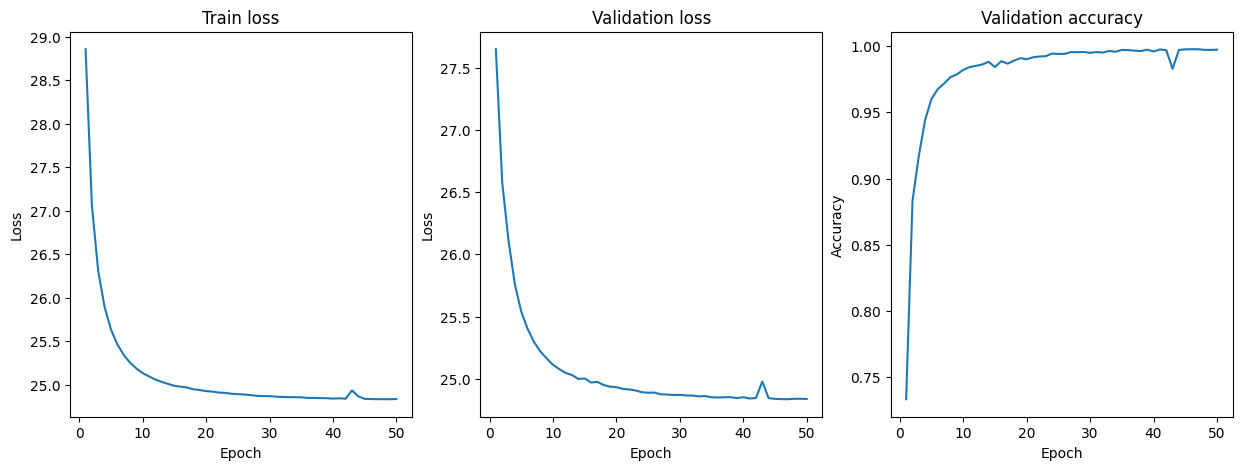
\includegraphics[width=\textwidth]{figures/no-residual-train-curves.png}
        \caption{Train and loss curves for the MLP without any residual streams.}
        \label{fig:nr-train-curves}
    \end{subfigure}

    \begin{subfigure}{0.9\textwidth}
        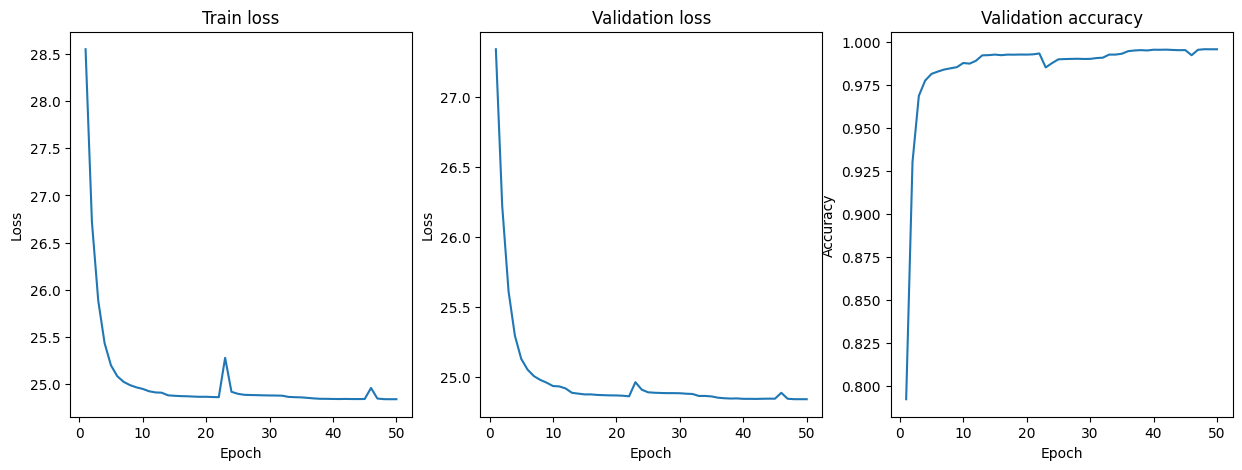
\includegraphics[width=\textwidth]{figures/residual-train-curves.png}
        \caption{Train and loss curves for the MLP with a residual stream per layer.}
        \label{fig:r-train-curves}
    \end{subfigure}

    \begin{subfigure}{0.9\textwidth}
        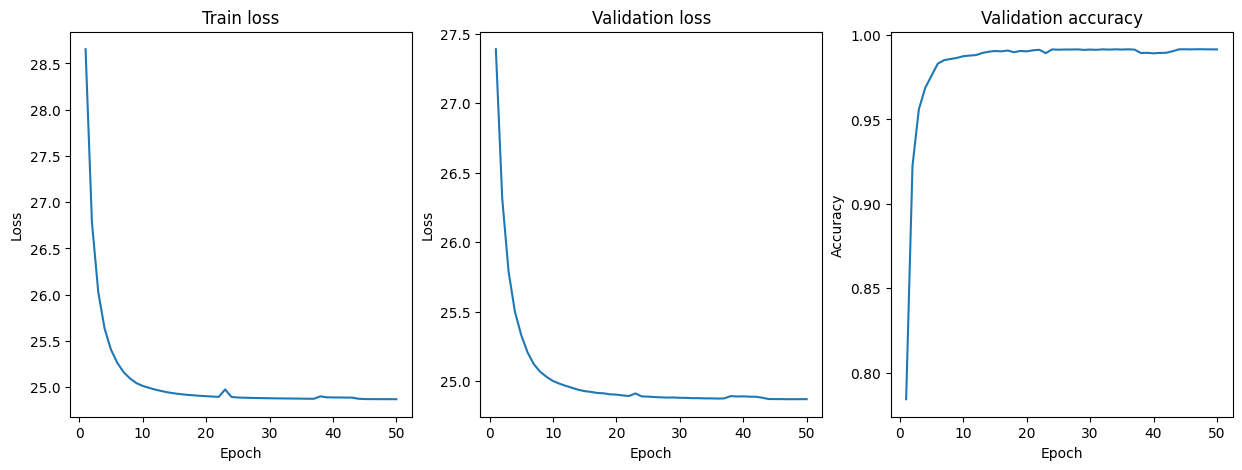
\includegraphics[width=\textwidth]{figures/single-residual-train-curves.png}
        \caption{Train and loss curves for the MLP with a single residual stream from input to layer-norm.}
        \label{fig:sr-train-curves}
    \end{subfigure}
\end{figure}

\cref{fig:nr-train-curves,fig:r-train-curves,fig:sr-train-curves} show the train curves for the different models.
All of these eventually reach near 100\% accuracy.
The best model is chosen based on best validation accuracy and is chosen on the first instance of the best validation loss.

\begin{figure}
    \centering
    \begin{subfigure}{0.9\textwidth}
        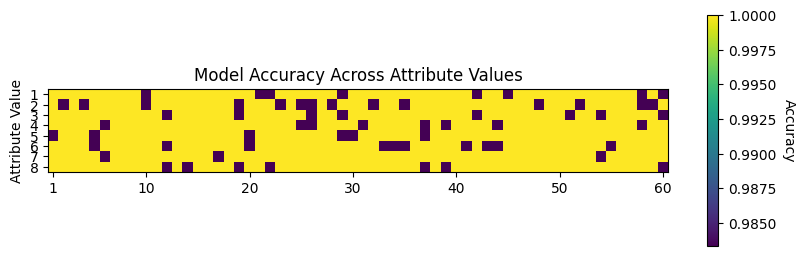
\includegraphics[width=\textwidth]{figures/no-residual-accuracy.png}
        \caption{The accuracy of the non-residual model on each attribute value.}
        \label{fig:nr-accuracy}
    \end{subfigure}
    \begin{subfigure}{0.9\textwidth}
        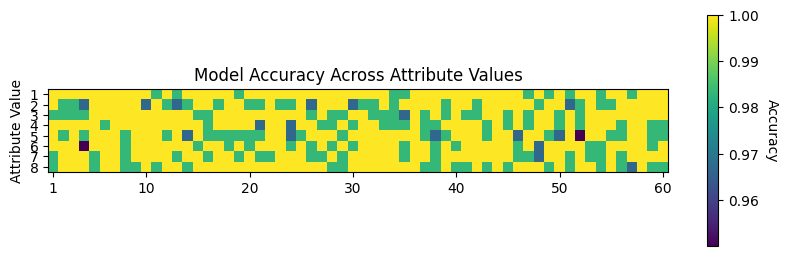
\includegraphics[width=\textwidth]{figures/residual-accuracy.png}
        \caption{The accuracy of the full residual model on each attribute value.}
        \label{fig:r-accuracy}
    \end{subfigure}
    \begin{subfigure}{0.9\textwidth}
        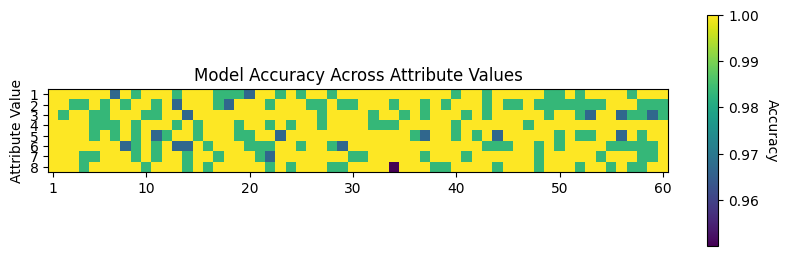
\includegraphics[width=\textwidth]{figures/single-residual-accuracy.png}
        \caption{The accuracy of the single residual model on each attribute value.}
        \label{fig:sr-accuracy}
    \end{subfigure}
\end{figure}

\cref{fig:nr-accuracy,fig:r-accuracy,fig:sr-accuracy} show the accuracy of the model across all attributes and their values.
All other values are filled with a uniform random attribute.
All fills are presented to show that there is no bias towards a particular fill value.

From these plots I am fairly confident that my setup for the dataset and the training of the model is sound though there are clearly differences between how the residual streams are applied.

\section{Steering adaptor}

A forward hook is inserted at the 256-dim layer to extract activations for the contrastive pairs.
In the case of the residual stream per layer model the hook is inserted after the residual stream.

The inputs for generating the contrastive pairs are made as

\begin{itemize}[nolistsep]
    \item Selecting one attribute to target steering.
    \item Positive examples set this attribute to 0.
    \item Negative examples set this attribute to 1-7.
\end{itemize}

CAA simply takes the difference of means of these two activations as a steering vector.
A forward hook is registered at the same 256-dim layer which simply adds the scaled (parameterised by $\lambda$) steering vector to the output and returns it for the next layer.

To get repeated runs, a set of attributes is chosen\footnote{For ease of implementation these are just the first $n$ attributes} and the above process is applied to each.
In the end I run 20 repeats.

\begin{figure}
    \centering
    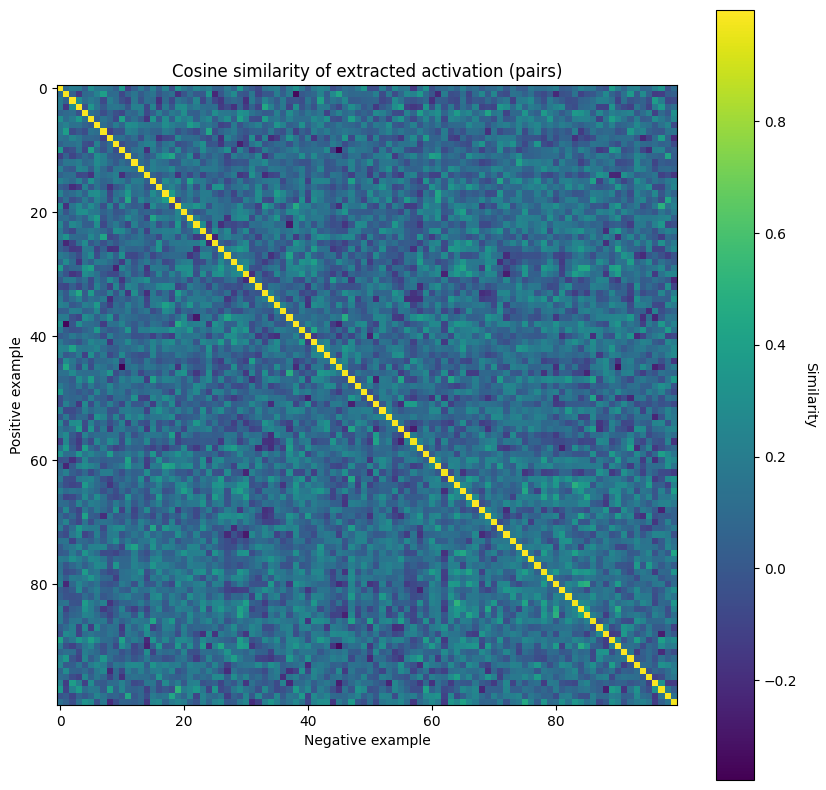
\includegraphics[width=0.9\textwidth]{figures/cosine-similarity.png}
    \caption{The cosine similarity between a sample of positive and negative pairs. This is for a specific attribute.}
    \label{fig:cosine-similarity}
\end{figure}

Figure \ref{fig:cosine-similarity} shows the cosine similarity of a sample of attributes.
The similarity between pairs is very high as expected as the other 59 attributes are identical.
The cross similarity is much lower showing that there is a variety of examples that are present when training the adaptor.
This plot is essentially the same across the models with minor differences in the exact similarity values.

\begin{figure}
    \centering
    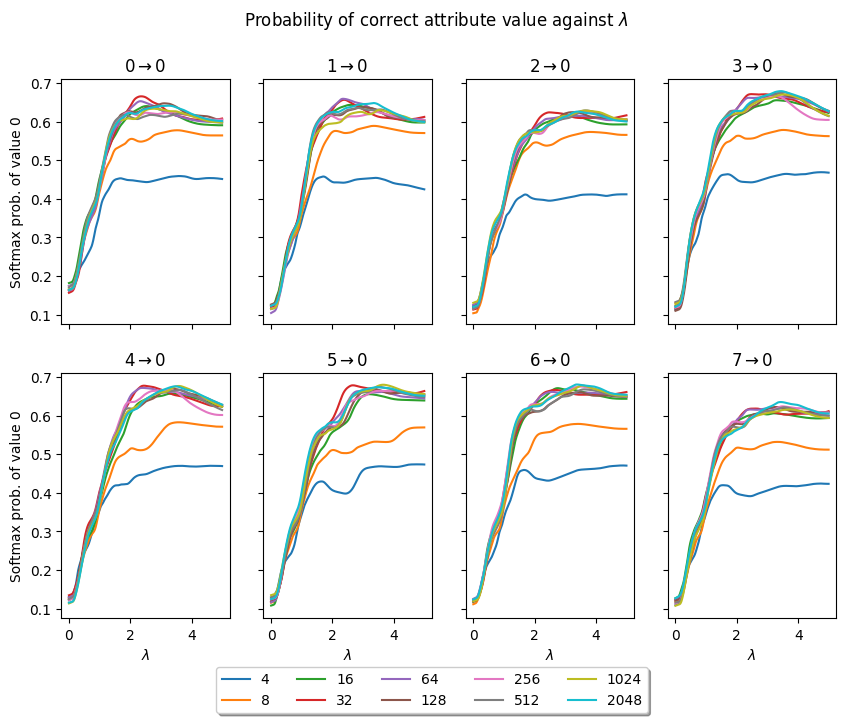
\includegraphics[height=0.4\textheight]{figures/no-residual-steering.png}
    \caption{The softmax probability of the target label (0) given the input label as a function of the scaling parameter $\lambda$. This is the model without any residual streams.}
    \label{fig:nr-steering}
\end{figure}

\begin{figure}
    \centering
    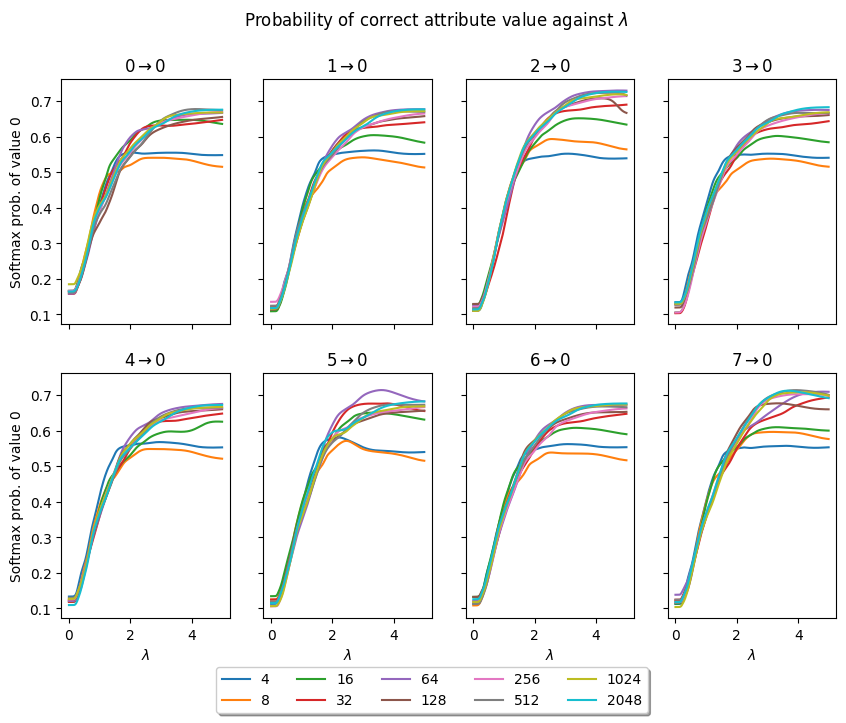
\includegraphics[height=0.4\textheight]{figures/residual-steering.png}
    \caption{The softmax probability of the target label (0) given the input label as a function of the scaling parameter $\lambda$. This is the model with a residual streams per layer.}
    \label{fig:r-steering}
\end{figure}

\begin{figure}
    \centering
    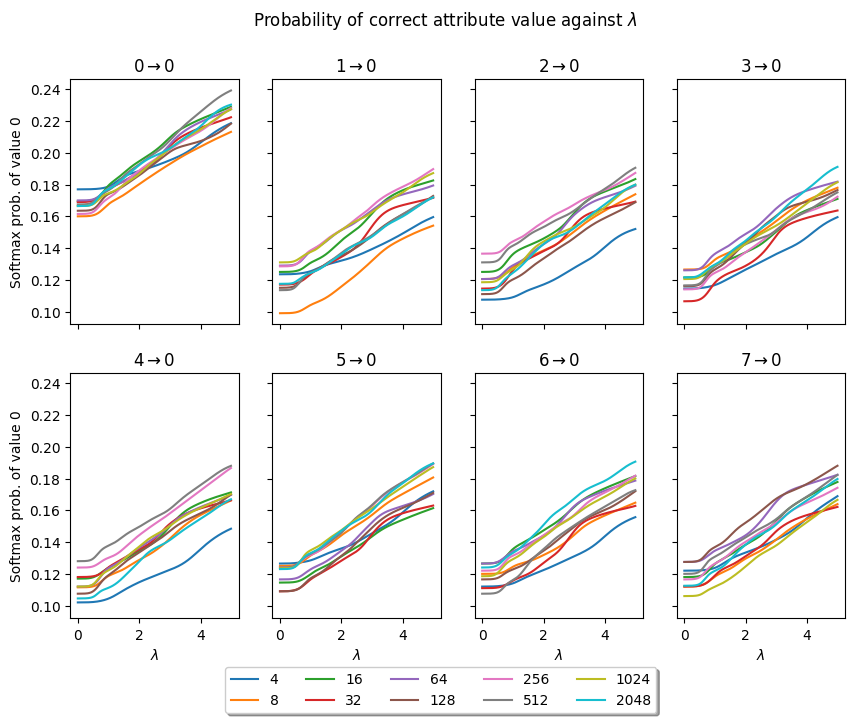
\includegraphics[height=0.4\textheight]{figures/single-residual-steering.png}
    \caption{The softmax probability of the target label (0) given the input label as a function of the scaling parameter $\lambda$. This is the model with a single residual stream from input to layernorm.}
    \label{fig:sr-steering}
\end{figure}

\cref{fig:nr-steering,fig:r-steering} demonstrate the effect of the CAA steering on the different attribute values for the target attribute.
The remaining attribute values are randomly selected.
The experiment is run over a range of example values for each 20 repeats and for each experiment the mean over 100 test inputs is returned.

Clearly demonstrated is that 4 and 8 examples do not achieve the same efficacy as the other examples regardless of the strength of the steering vector.
This does not take into account the effect on the attributes nor the softmax prob of the other values.
These experiments demonstrate that the steering vectors are able to steer effectively.

\section{Steering metric}

A subset of 1000 of the contrastive pairs above are withheld during training.
The negative generating inputs are fed through the model with the trained steering adaptor and the output recorded.
The goal is for the output to match the positive generating labels.

There are two metrics that I test:
\begin{itemize}[nolistsep]
    \item The accuracy on the steered attribute alone.
    \item The accuracy on all the attributes (this is the one stated in the paper).
\end{itemize}

\begin{figure}
    \centering
    \begin{subfigure}{0.45\textwidth}
        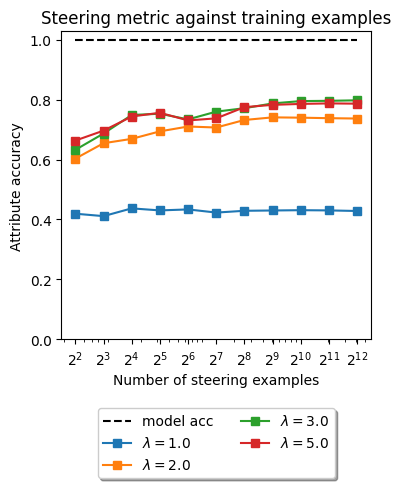
\includegraphics[width=\textwidth]{figures/no-residual-reproduction.png}
        \caption{Standard model steering accuracy on the steered attribute alone.}
        \label{fig:nr-reproduction}
    \end{subfigure}
    \hfill
    \begin{subfigure}{0.45\textwidth}
        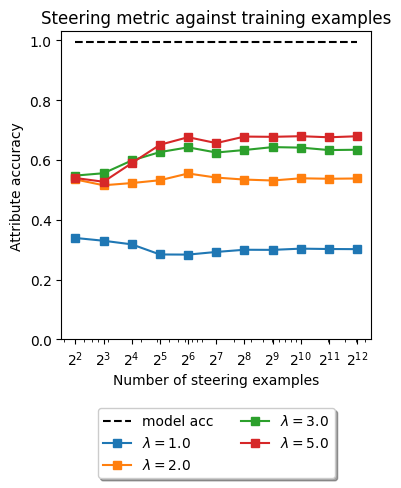
\includegraphics[width=\textwidth]{figures/residual-reproduction.png}
        \caption{Residual model steering accuracy on the steered attribute alone.}
        \label{fig:r-reproduction}
    \end{subfigure}
    \begin{subfigure}{0.45\textwidth}
        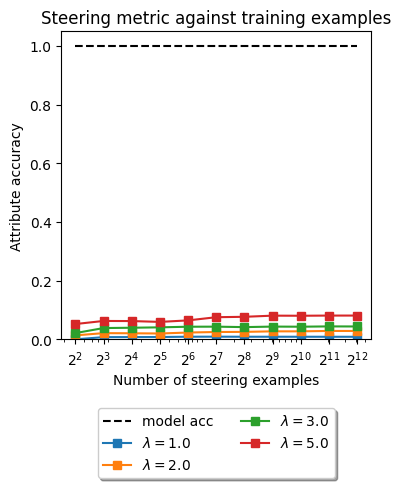
\includegraphics[width=\textwidth]{figures/single-residual-reproduction.png}
        \caption{Single residual stream model steering accuracy on the steered attribute alone.}
        \label{fig:sr-reproduction}
    \end{subfigure}
\end{figure}

\cref{fig:nr-reproduction,fig:r-reproduction,fig:sr-reproduction} show the attempt at reproducing the paper figures for the top-left plot in Figure 1.
This only focuses on the CAA approach.
This uses a different metric to the paper focusing only on attribute accuracy rather than total accuracy and the trends are similar to those in the paper.
However, these plots are still not the same as the papers plots especially as they do not use the same metric.

\begin{figure}
    \centering
    \begin{subfigure}{0.45\textwidth}
        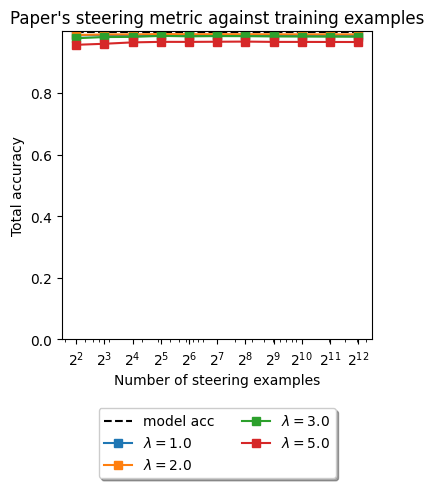
\includegraphics[width=\textwidth]{figures/no-residual-full-reproduction.png}
        \caption{Standard model steering accuracy on the steered attribute alone.}
        \label{fig:nr-correct}
    \end{subfigure}
    \hfill
    \begin{subfigure}{0.45\textwidth}
        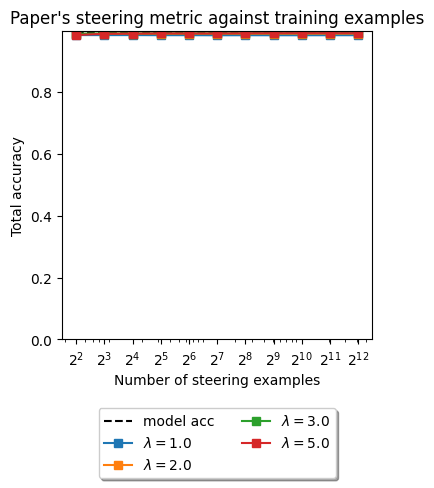
\includegraphics[width=\textwidth]{figures/residual-full-reproduction.png}
        \caption{Residual model steering accuracy on the steered attribute alone.}
        \label{fig:r-correct}
    \end{subfigure}
    \begin{subfigure}{0.45\textwidth}
        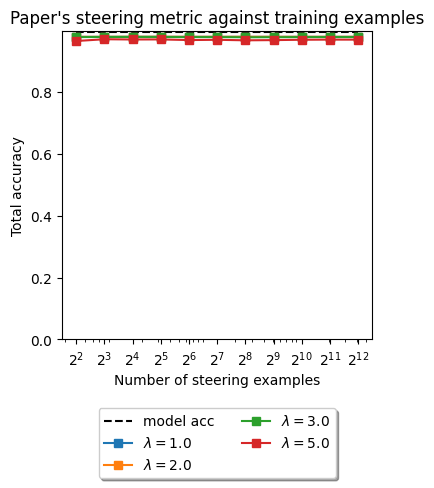
\includegraphics[width=\textwidth]{figures/single-residual-full-reproduction.png}
        \caption{Single residual stream model steering accuracy on the steered attribute alone.}
        \label{fig:sr-correct}
    \end{subfigure}
\end{figure}

\cref{fig:nr-correct,fig:r-correct,fig:sr-correct} show the reproduction using the stated steering metric of total accuracy across all target labels.

\chapter{Layer Sweeps}

\emph{This chapter includes the figures generated when running the experiments across all 11 layers of GPT-2 small \citep{saelens}.}
\emph{It is important to note that the exact metrics presented in \cref{sec:prompt-pairs} are not used here.}
\emph{Instead the absolute SAE activation values are used to better get a sense of how strongly the adaptors are effecting the model.}

\emph{Only CAA is presented here as a proxy for the other runs and to save pages.}
\emph{The ideal choice of layer was found to be layer 7, discussion of the figures will not be carried out due to the number of figures presented.}

\begin{figure}
    \centering
        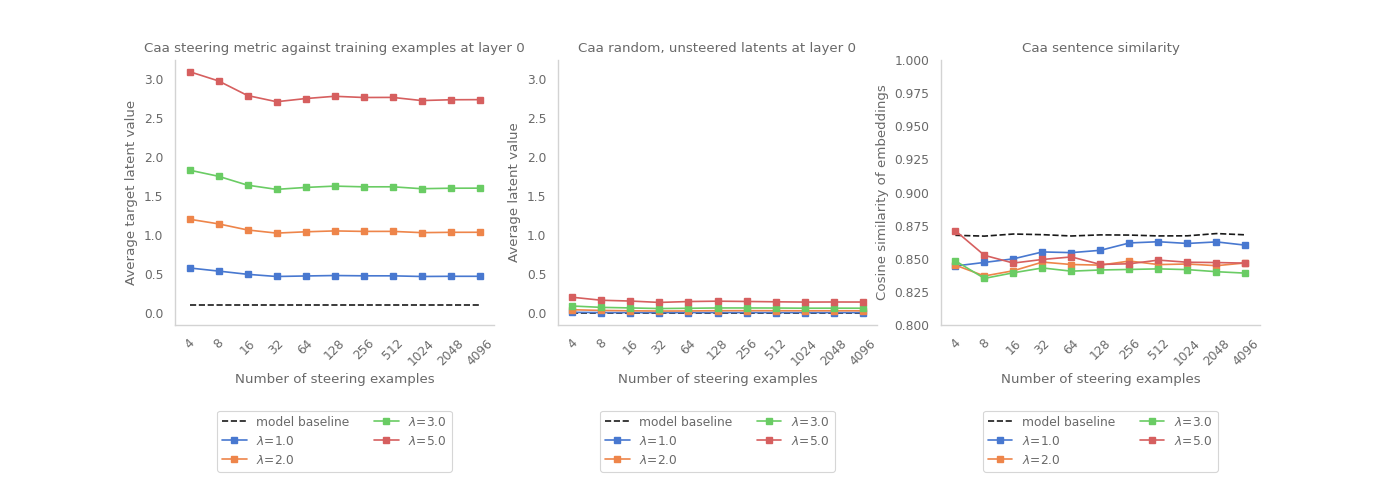
\includegraphics[width=\textwidth]{figures/gpt2_sweep_0.png}
        \label{fig:0}
\end{figure}

\begin{figure}
    \centering
        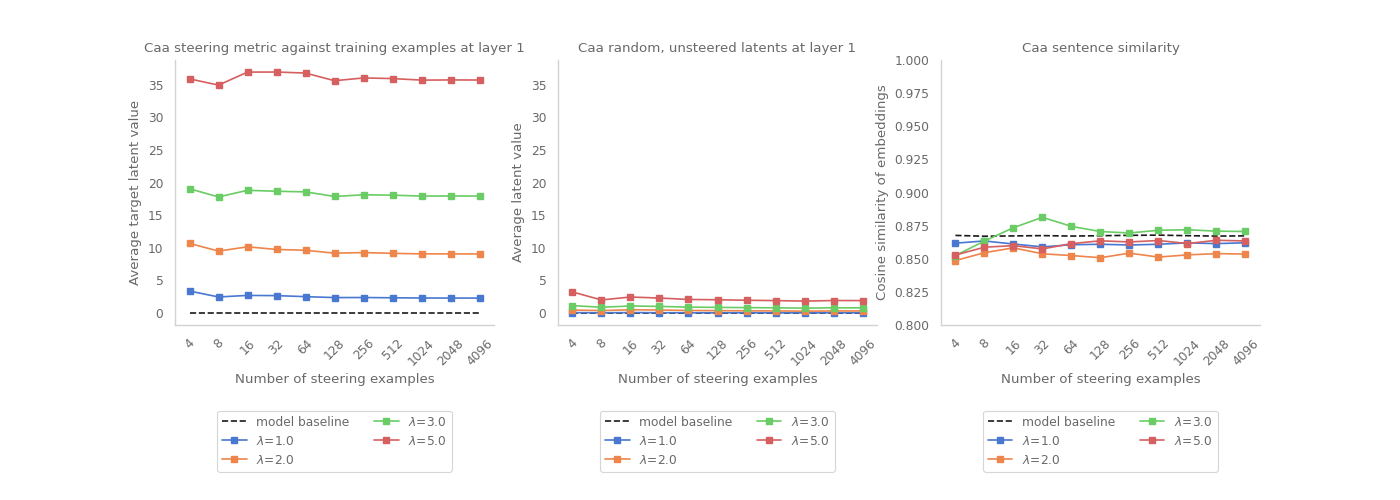
\includegraphics[width=\textwidth]{figures/gpt2_sweep_1.png}
        \label{fig:1}
\end{figure}

\begin{figure}
    \centering
        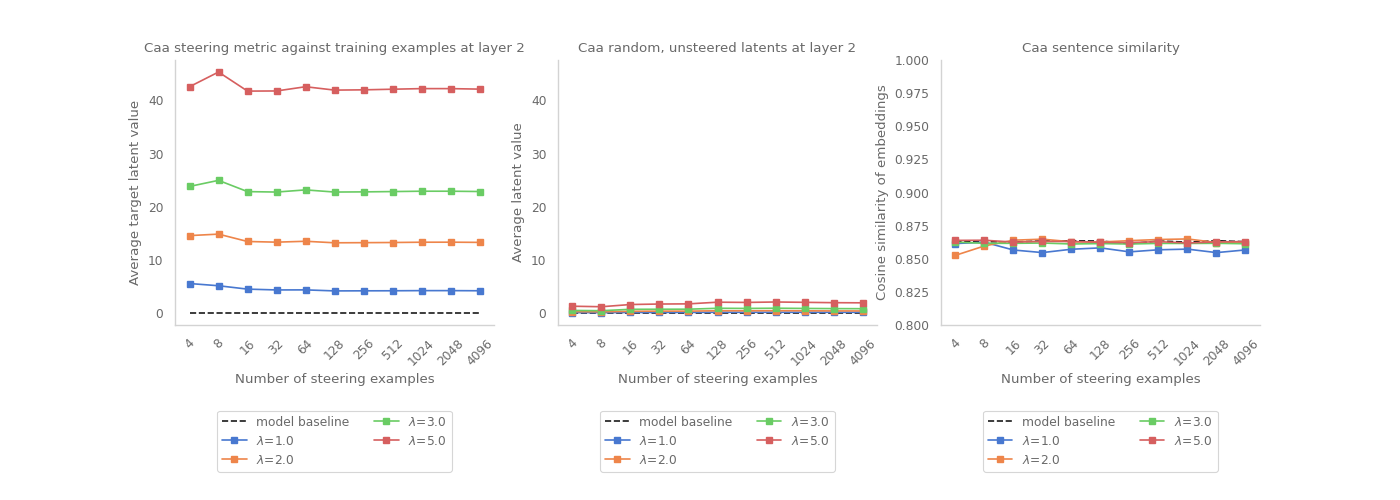
\includegraphics[width=\textwidth]{figures/gpt2_sweep_2.png}
        \label{fig:2}
\end{figure}

\begin{figure}
    \centering
        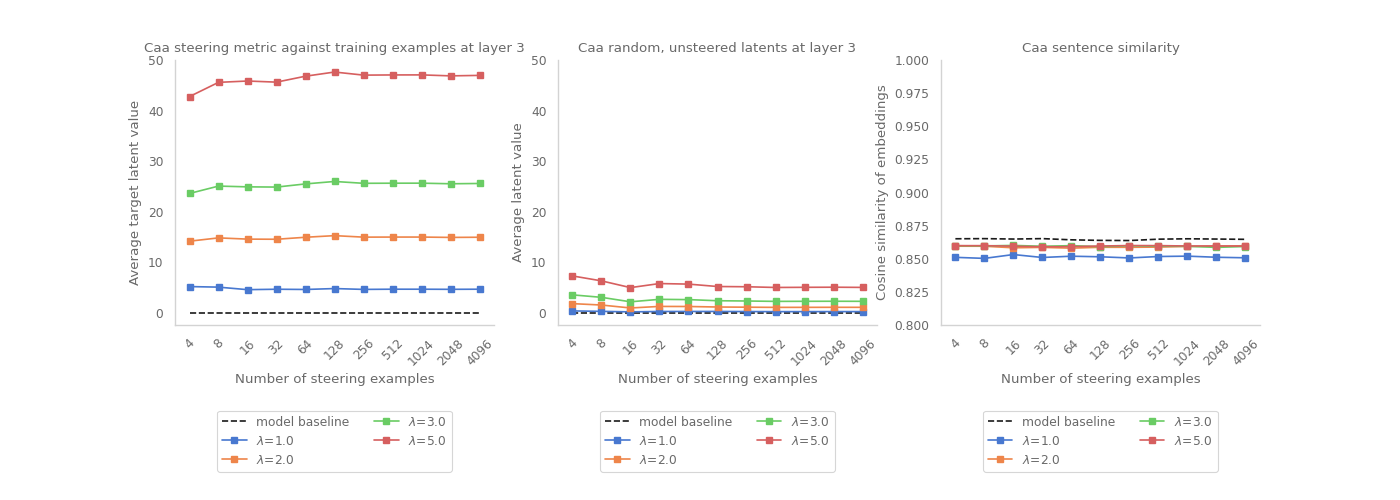
\includegraphics[width=\textwidth]{figures/gpt2_sweep_3.png}
        \label{fig:3}
\end{figure}

\begin{figure}
    \centering
        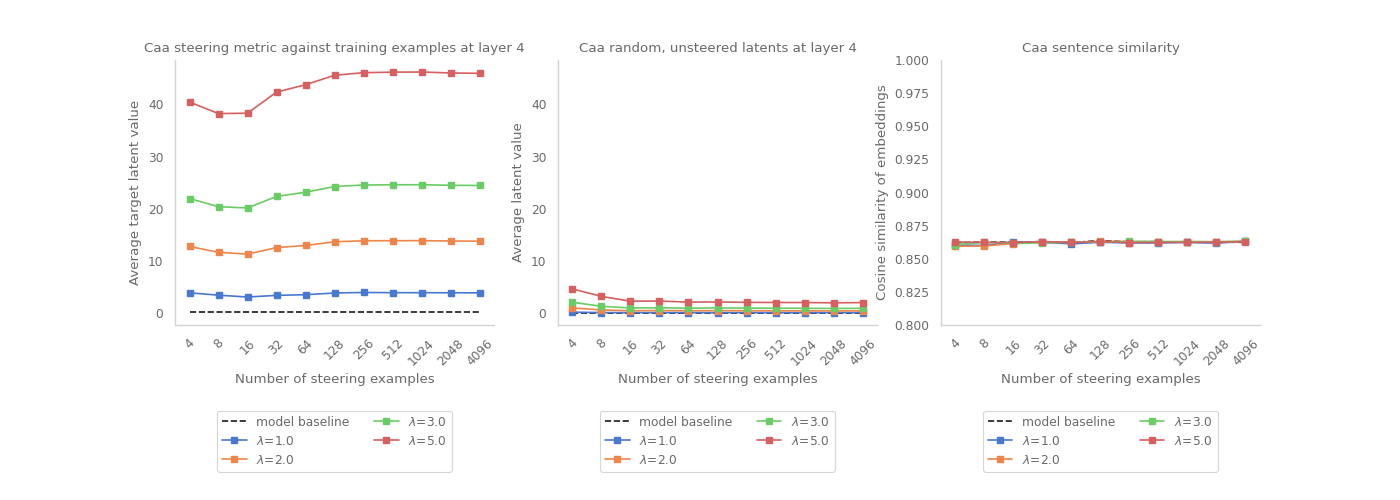
\includegraphics[width=\textwidth]{figures/gpt2_sweep_4.png}
        \label{fig:4}
\end{figure}

\begin{figure}
    \centering
        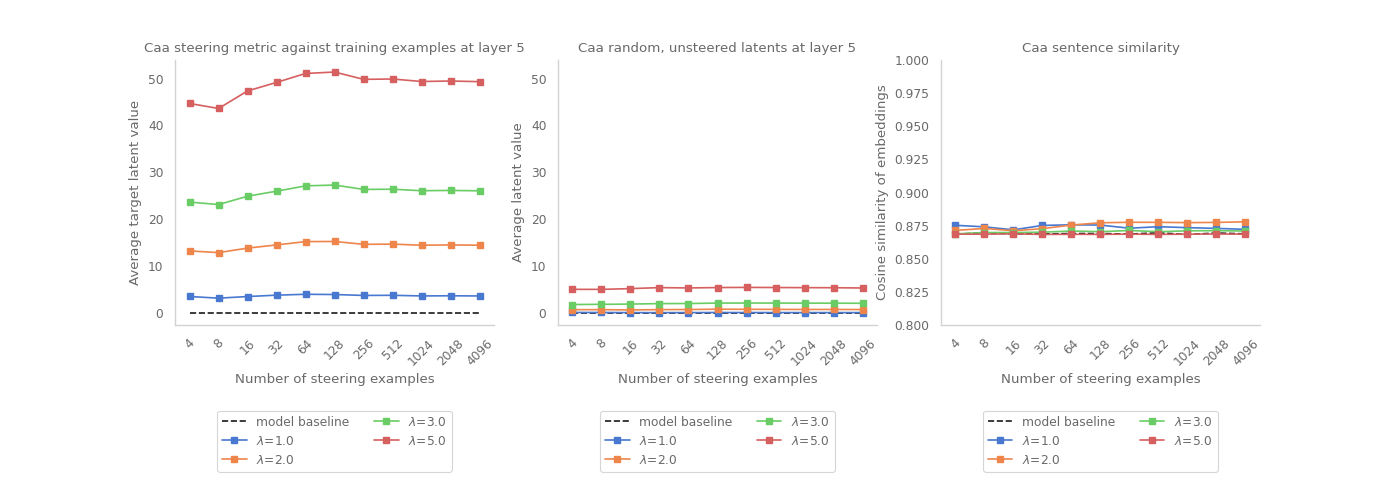
\includegraphics[width=\textwidth]{figures/gpt2_sweep_5.png}
        \label{fig:5}
\end{figure}

\begin{figure}
    \centering
        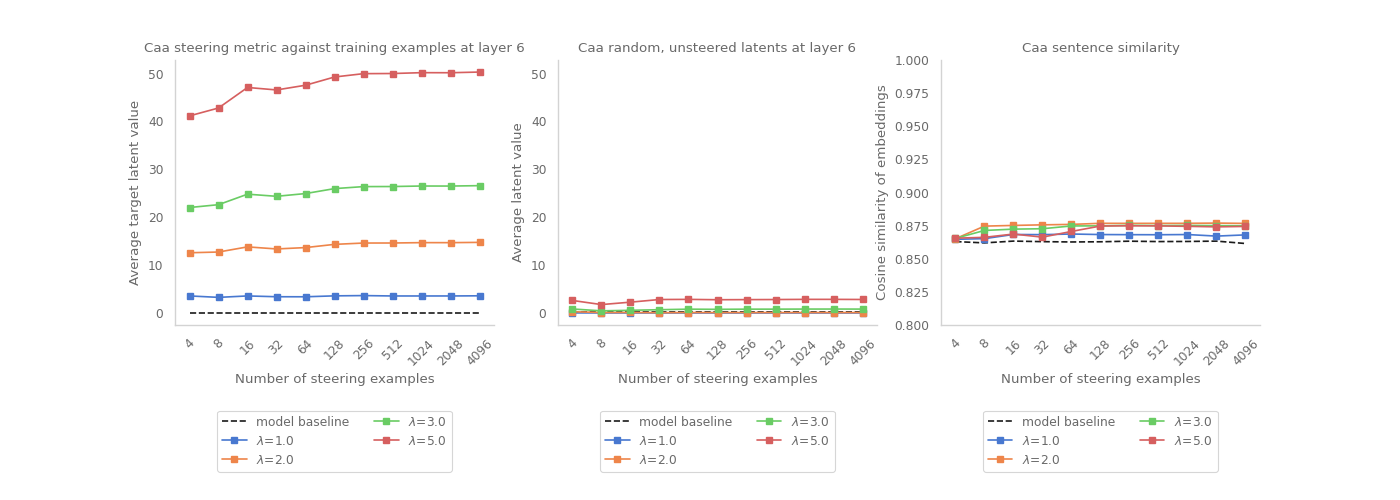
\includegraphics[width=\textwidth]{figures/gpt2_sweep_6.png}
        \label{fig:6}
\end{figure}

\begin{figure}
    \centering
        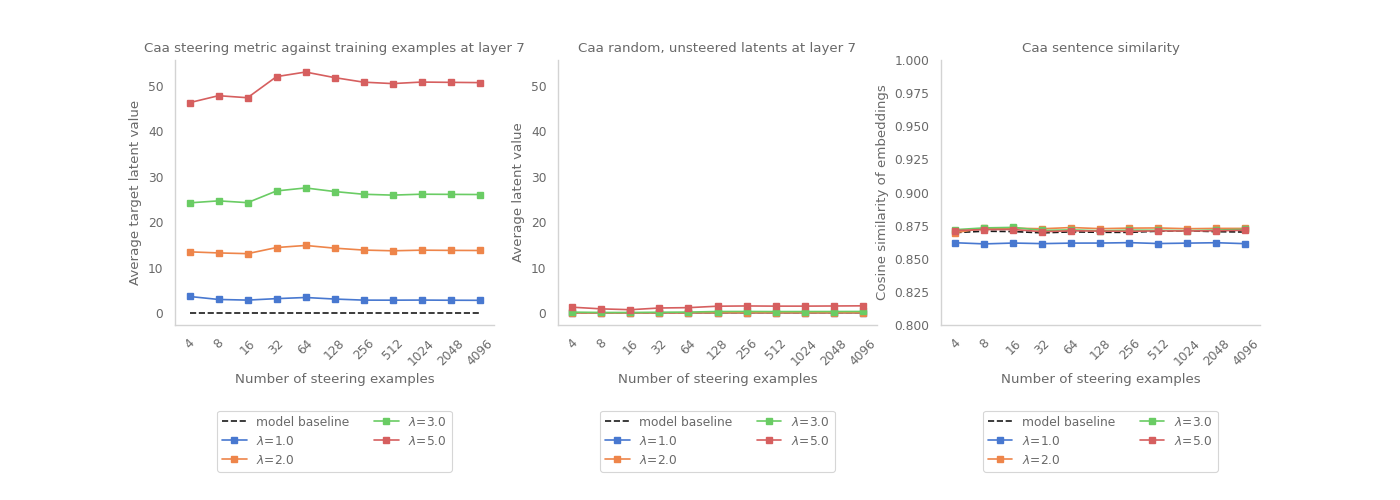
\includegraphics[width=\textwidth]{figures/gpt2_sweep_7.png}
        \label{fig:7}
\end{figure}

\begin{figure}
    \centering
    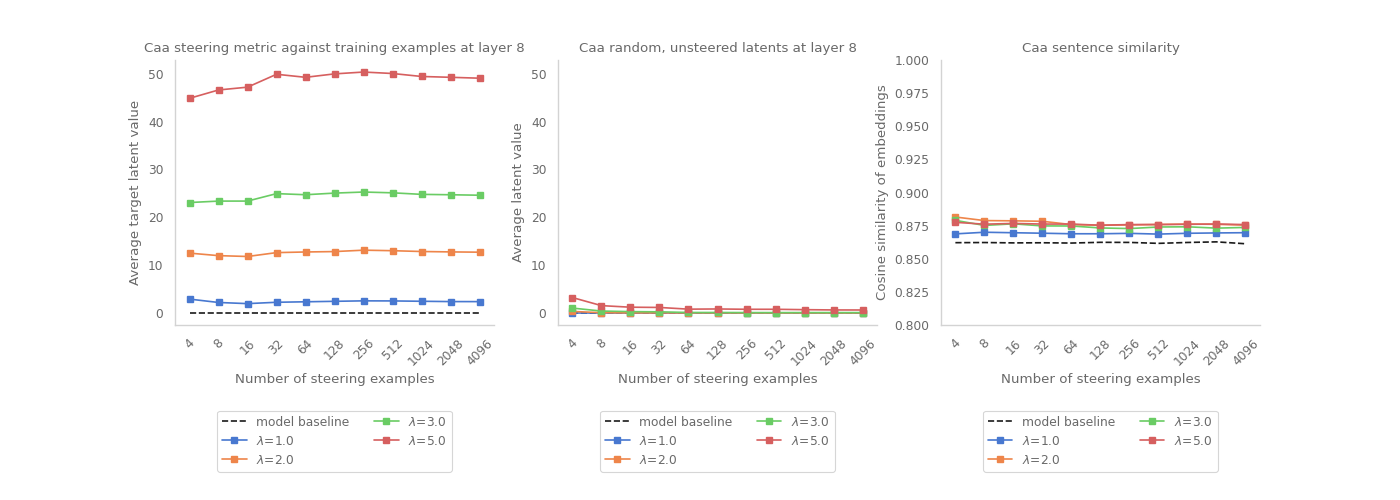
\includegraphics[width=\textwidth]{figures/gpt2_sweep_8.png}
    \label{fig:8}
\end{figure}

\begin{figure}
    \centering
        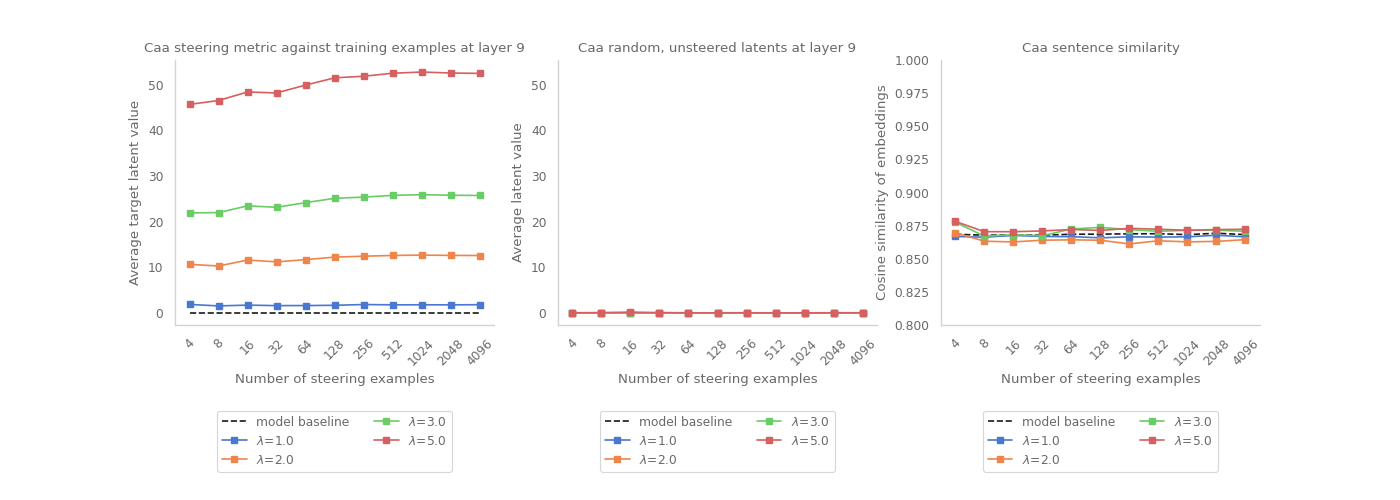
\includegraphics[width=\textwidth]{figures/gpt2_sweep_9.png}
        \label{fig:9}
\end{figure}

\begin{figure}
    \centering
        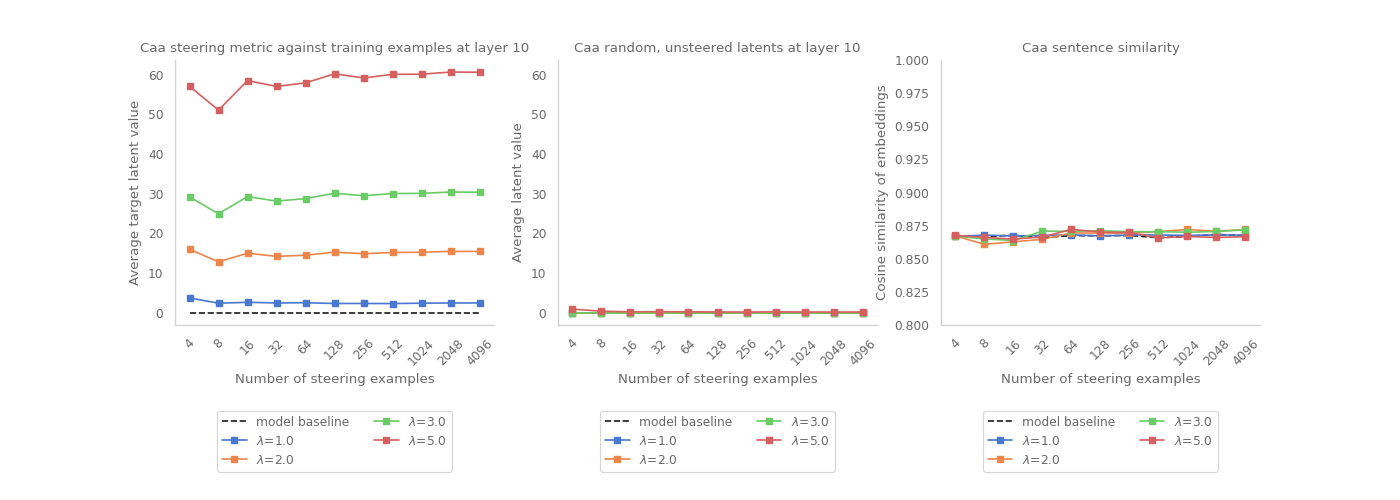
\includegraphics[width=\textwidth]{figures/gpt2_sweep_10.png}
        \label{fig:10}
\end{figure}

\begin{figure}
    \centering
    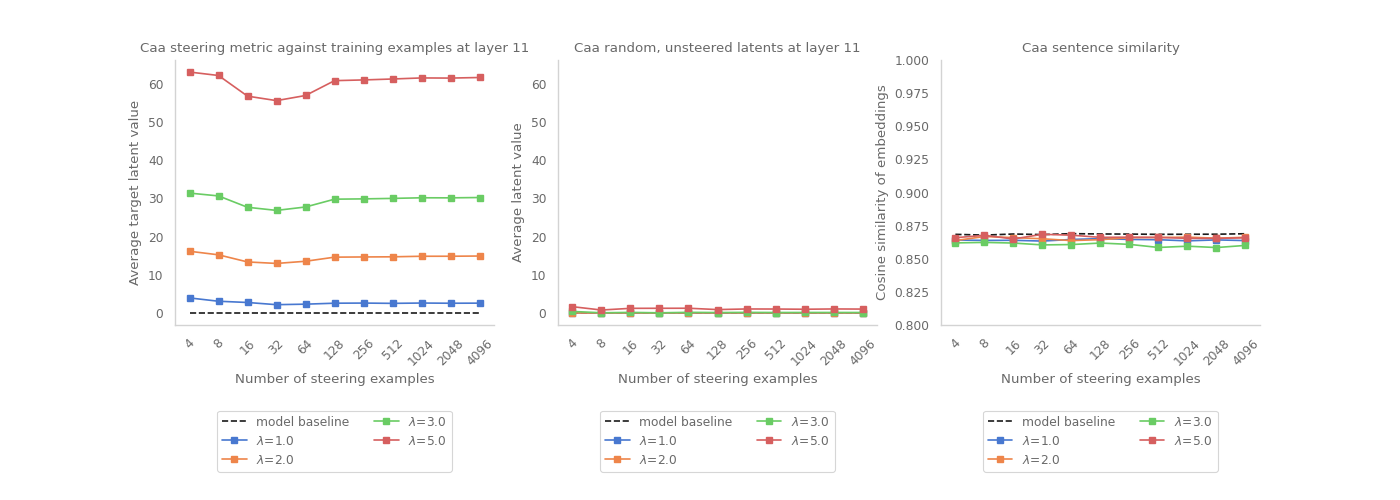
\includegraphics[width=\textwidth]{figures/gpt2_sweep_11.png}
    \label{fig:11}
\end{figure}

%TC:endignore

\end{document}
